% ----------------------------------------------------------------
% achemso --- Support for submissions to American Chemical
%  Society journals
% Maintained by Joseph Wright
% E-mail: joseph.wright@morningstar2.co.uk
% Originally developed by Mats Dahlgren
%  (c) 1996-98 by Mats Dahlgren
%  (c) 2007-2008 Joseph Wright
% Released under the LaTeX Project Public license v1.3c or later
% See http://www.latex-project.org/lppl.txt
% 
% Part of this bundle is derived from cite.sty, to which the
% following license applies:
%   Copyright (C) 1989-2003 by Donald Arseneau
%   These macros may be freely transmitted, reproduced, or
%   modified provided that this notice is left intact.
% ----------------------------------------------------------------
% 
% The achemso bundle provides a LaTeX class file and BibTeX style
% file in accordance with the requirements of the American
% Chemical Society.  The files can be used for any documents, but
% have been carefully designed and tested to be suiTable for
% submission to ACS journals.
% 
% The bundle also includes the natmove package.  This package is
% loaded by achemso, and provides automatic moving of superscript
% citations after punctuation.

\documentclass[
%journal=ancac3, % for ACS Nano
%journal=acbcct, % for ACS Chem. Biol.
journal=jpcbfk, % for undefined journal
manuscript=article]{achemso}
\oddsidemargin= 0.25 in
\evensidemargin= 0.25 in


\usepackage[version=3]{mhchem} % Formula subscripts using \ce{}
\usepackage{graphicx}
\usepackage{caption}
\usepackage{subcaption}
\usepackage[labelfont={bf}]{caption}
\usepackage{minted}
\usepackage[export]{adjustbox}
\usepackage{multicol} 
\usepackage[euler]{textgreek}
\let\titlefont\undefined
\usepackage[fontsize=10pt]{scrextend}
\usepackage{wrapfig}
\usepackage [english]{babel}
\usepackage [autostyle, english = american]{csquotes}
\MakeOuterQuote{"}

\SectionNumbersOn 

\pagenumbering{roman}
\author{Kasidet (Jing) Trerayapiwat}
\email{jing_sk129@hotmail.com}
\affiliation[Bowdoin College]
{An Honors Thesis for the Department of Chemistry \linebreak \linebreak Bowdoin College, 2016 \\ \copyright 2016 Kasidet Trerayapiwat}


\title[\texttt{achemso} demonstration]
{Benchmarking Ab Initio Computational Methods for the Quantitative Prediction of Sunlight-Driven Pollutant Degradation in Aquatic Environments}

\begin{document}
	\begin{abstract}
		Understanding the changes in molecular electronic structure following the absorption of light is a fundamental challenge for the goal of predicting photochemical rates and mechanisms. Proposed here is a systematic benchmarking method to evaluate accuracy of a model to quantitatively predict photo-degradation of small organic molecules in aquatic environments. An overview of underlying computational theories relevant to understanding sunlight-driven electronic processes in organic pollutants is presented. To evaluate the optimum size of solvent sphere, molecular Dynamics and Time Dependent Density Functional Theory (MD-TD-DFT) calculations of an aniline molecule in different numbers of water molecules using CAM-B3LYP functional yielded excited state energy and oscillator strength values, which were compared with data from experimental absorption spectra. For the first time, a statistical method of comparing experimental and theoretical data is proposed. Underlying Gaussian functions of absorption spectra were deconvoluted and integrated to calculate experimental oscillator strengths. A Matlab code written by Soren Eustis was utilized to decluster MD-TD-DFT results. The model with 256 water molecules was decided to give the most accurate results with optimized computational cost and accuracy. MD-TD-DFT calculations were then performed on aniline, 3-F-aniline, 4-F-aniline, 3-Cl-aniline, 4-MeOacetophenone, and (1,3)-dimethoxybenzophenone with CAM-B3LYP, PBE0, M06-2X, LCBLYP, and BP86 functionals. BP86 functional was determined to be the best functional.	
		\end{abstract}
	
	\pagebreak
	\tableofcontents
	\pagebreak
	
	\pagenumbering{arabic}
	\setcounter{page}{1}
	\section{Introduction}
	
	\subsection{Environmental Photochemistry And Micropollutants}
	During the past century, more and more synthetic chemicals have been created for commercial pharmaceuticals and personal care products. Each year, about 300 million tons of organic chemicals are being added into water systems from household septics, waste water facilities, and many other paths.\cite{Schwarzenbach2006} These chemicals have been detected in ng/L to μg/L quantity in natural water bodies: rivers, lakes, and the oceans.\cite{Monteiro2010} The amount of chemicals being introduced into the water raises the need to understand the consequences of these compounds. If the water is polluted, eventually animals, human, and other living beings in this world are affected. For example, in 1956, Minamata disease was identified to be caused by consumption of fish bio-accumulated by methylmercury from a nearby chemical factory.\cite{Harada1995} While some major toxic chemicals, such as mercury, \ce{CCl4}, DDT, etc., have been constantly regulated or banned by governments for their effects on agriculture and the environment, many more chemical wastes have not been studied and regulated to the same degree. Even though some chemicals are approved as safe for daily usage in household products, their impacts after being disposed into water remain largely unknown. These low-concentration chemicals are collectively called micropollutants.\cite{Schwarzenbach2006} The small concentration, large number of different species in water, and difficulty of separating or concentrating them for analysis all retard the effort to understand their effects on in water systems. These are "The Challenge of Micropollutants in Aquatic Systems".\cite{Schwarzenbach2006}
	\begin{wrapfigure}{r}{0.5\textwidth}
		\centering	
		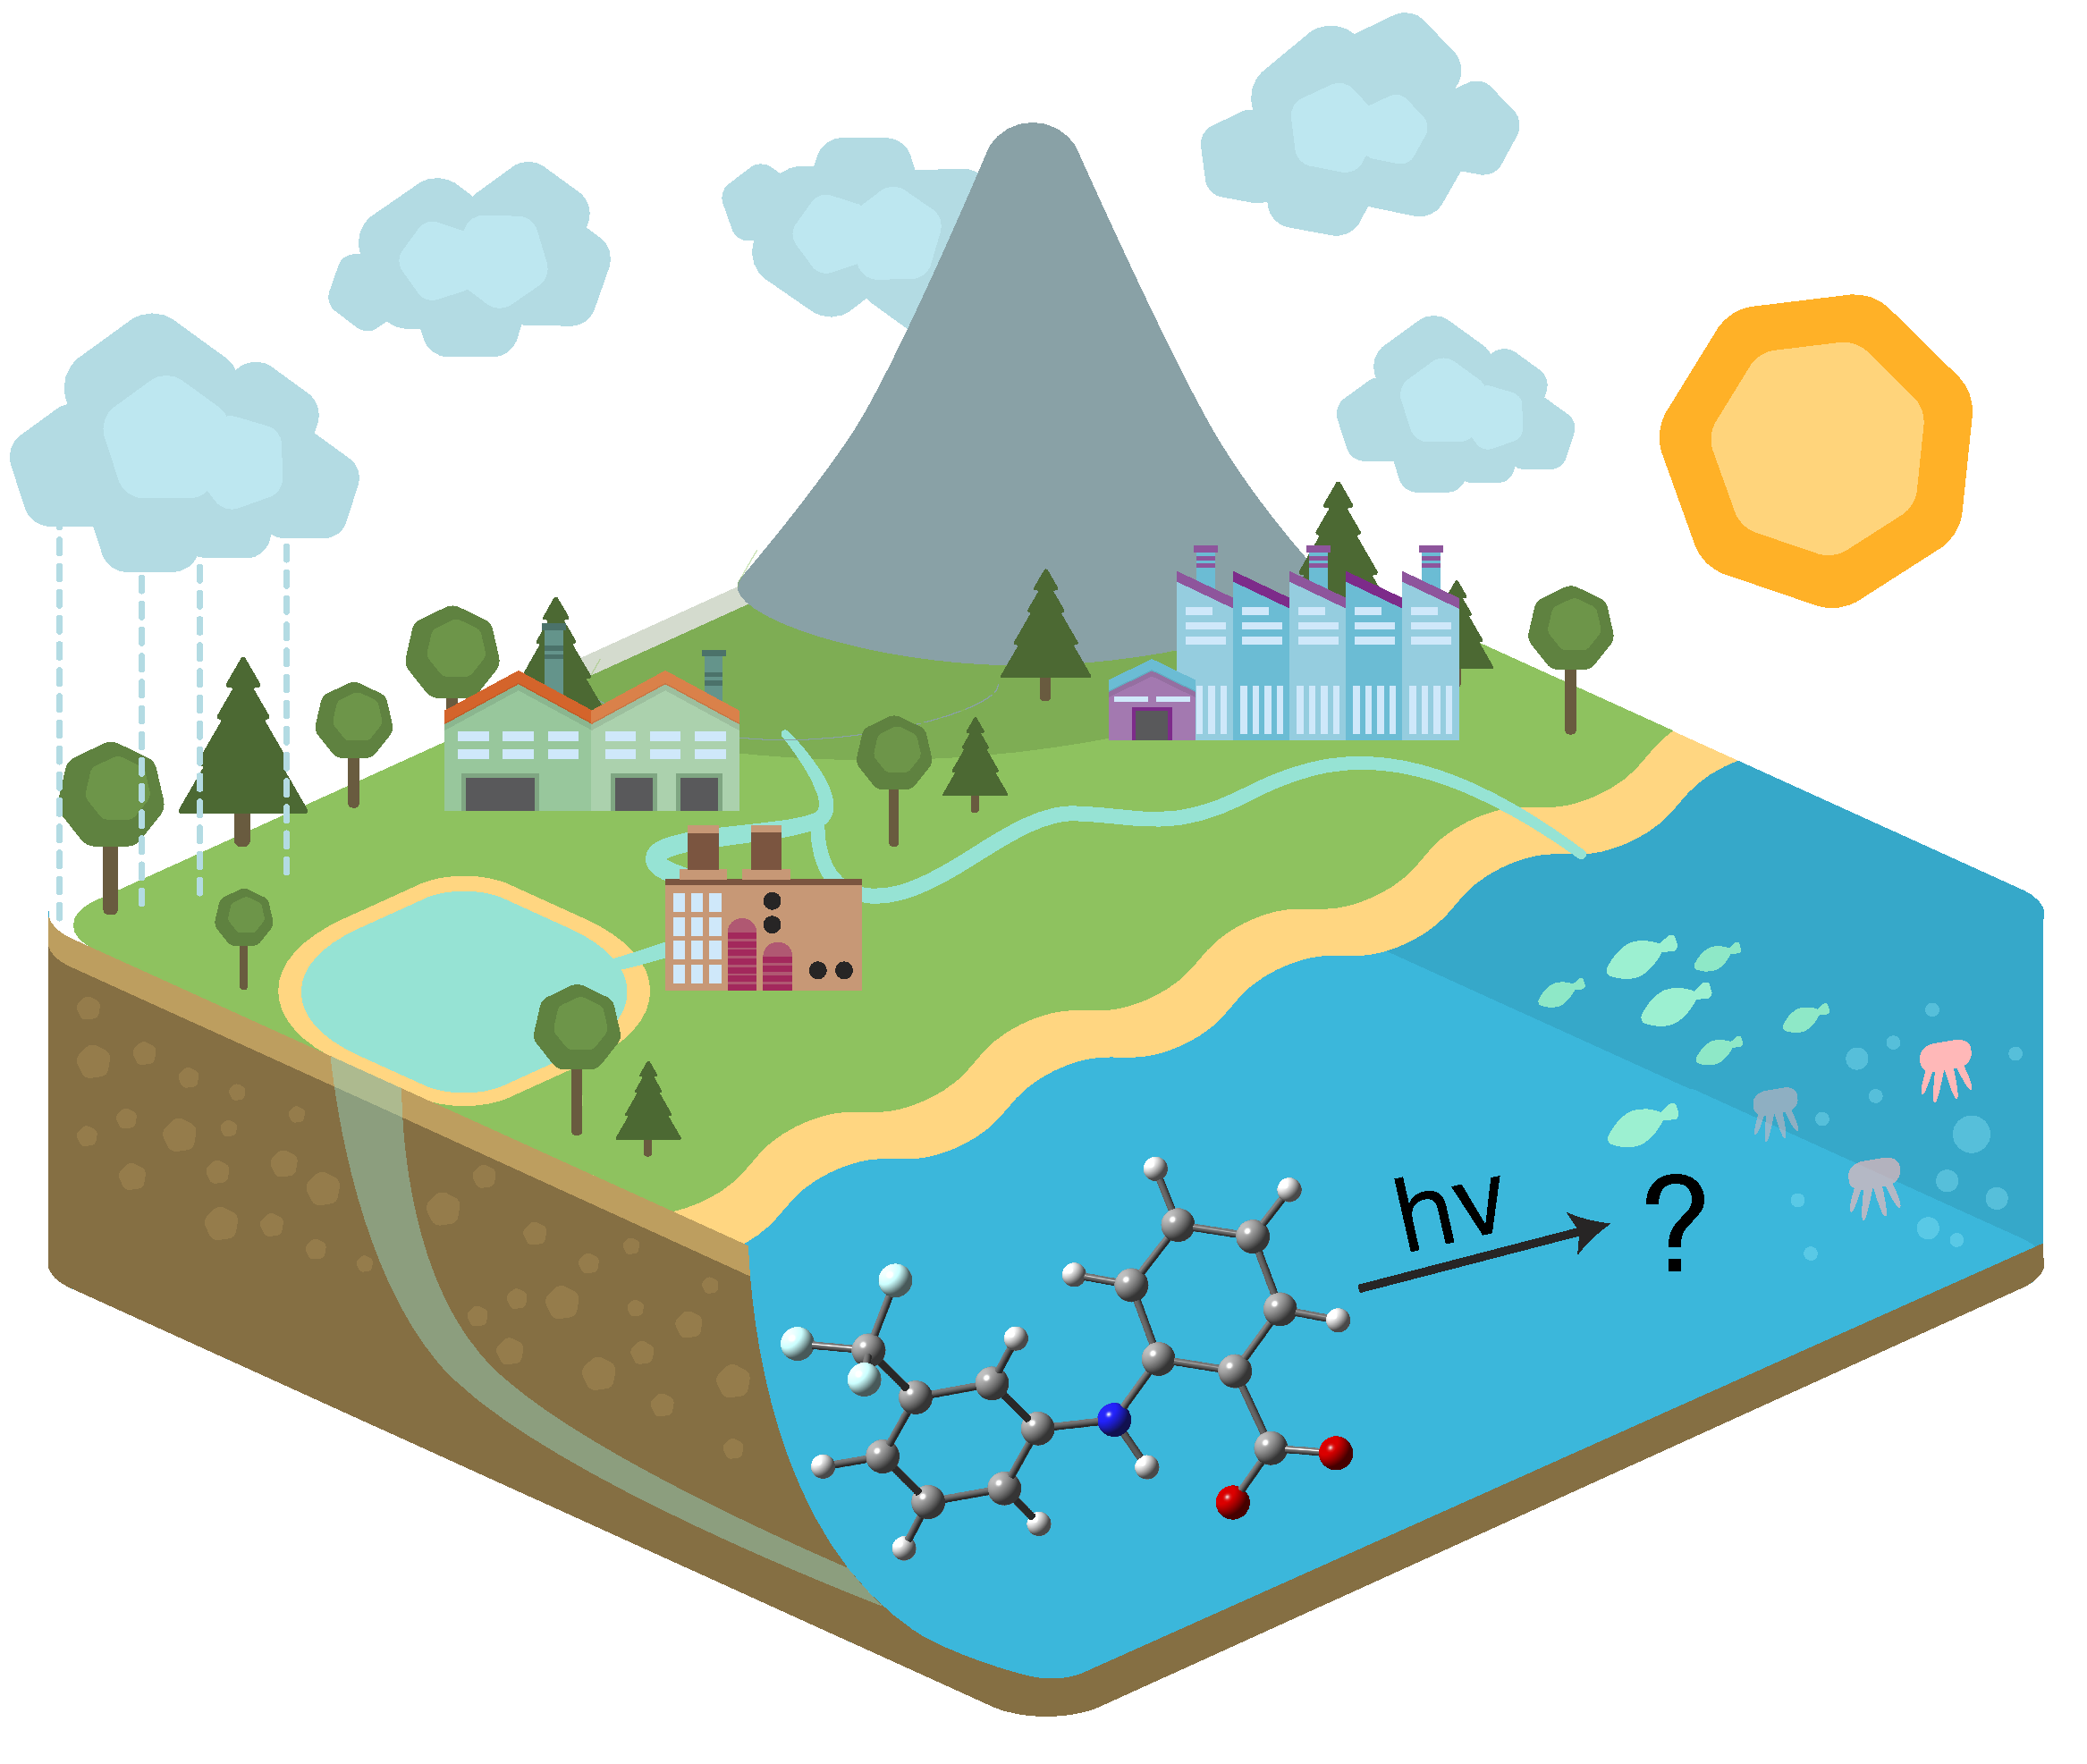
\includegraphics[width=0.48\textwidth]{images/waterCycleDiagram2_mod.pdf}
		\caption{Environmental fate of micropollutants in water. Under sunlight, molecules can undergo unknown photo-reactions to form unknown products.\cite{noodledoodle}}\label{fig:waterFluff}
		\vspace{-15pt}
	\end{wrapfigure}
	Since each individual species of micropollutant is not classified as harmful, major concerns of introducing them to water bodies are their reactions in water. In water with exposure to sunlight, photoreaction can occur as photons from the sun energize organic pollutants from ground state to excited state. In rivers close to discharge areas, photolysis has been confirmed to have direct connection to the observed attenuation in concentration of micropollutants from upstream to downstream.\cite{Conley2008,Daneshvar2010,Bonvin2011,Carlson2015} Observable decrease in concentrations means a significant portion of the pollutants undergo photo-reactions in exposure to sunlight. Eustis et al. carried out computational studies of triclosan in excited states.\cite{Kliegman2013}  Triclosan goes through photolysis under sunlight to form Dioxins and PCBs, well-known carcinogens.\cite{Bedoux2012} This is but one of many examples of large-scale, unintended consequences as a direct result of persistent, low-level concentrations of pollutants in aquatic ecosystems\cite{Morss2014}. One important step in triclosan's degradation process to its 4 major products is detachment of ortho-Cl from triclosan ring under 300 nm light. Confirmed by combining both experimental and computational results in the paper, ortho-chlorine photo-dissociates from triclosan through reductive cleavage pathway through biradical anion. Excited state bond energy of the breaking C-Cl reveals significantly smaller activation energy in reductive cleavage pathway compared to that of through homolytic mechanism. In this case, experimental method provides evidence of products from photo-reaction. Computational method provides reasons and insights into the microscopic world of atoms and electrons. Combing and analyzing results the two methods give a better understanding of photo-reactions in aquatic solutions. 
	
	\subsection{Photo-excitation and UV-VIS Spectrum}
	\begin{wrapfigure}{r}{0.5\textwidth}
		\centering	
		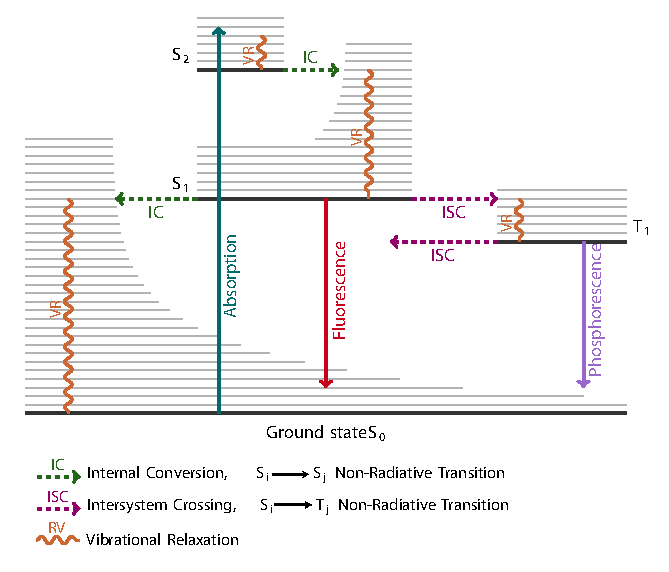
\includegraphics[width=0.48\textwidth]{images/jablonski.pdf}
		\caption{Jablonski diagram.\cite{Salvato-Vallverdu2009} A possible pathway of photo-excitation starts at ground state to singlet excited state, then triplet excited states.}\label{fig:jablonski}
		\vspace{-15pt}
	\end{wrapfigure}
	Understanding each step in the photochemically driven reaction is critical to properly evaluate the impact of a pollutant's
	environmental fate. The first, and most important step in this process is light absorption of ground state molecules to form chemically activated excited state molecules. A molecule in its ground state (S\textsubscript{0}) can absorb a photon to its first singlet excited state (S\textsubscript{1}), and then relax to its first triplet excited state (T\textsubscript{1}) as illustrated in Figure \ref{fig:jablonski}. Experimentally, studying absorption of photons in chemical compounds is done through UV-VIS absorption spectroscopy, followed by analysis of molar absorptivity and wavelength. In contrast to common misconception, a value of molar absorptivity is not a characteristic property of a compound. Molar absorptivity as a function of wavelength is highly dependent on the resolution used in the measurement.\cite{Hirayama2010}	
	\begin{figure}[!tbp]
		\centering
		\label{fig:PES}
		\begin{subfigure}[b]{0.48\textwidth}
			\includegraphics[width=1\textwidth]{images/PES1.pdf}
			\caption{}
			\label{fig:PESa)}
		\end{subfigure}
		\hfill
		\begin{subfigure}[b]{0.48\textwidth}
			\includegraphics[width=1\textwidth]{images/PES2.pdf}
			\caption{}
			\label{fig:PESb)}
		\end{subfigure}
		\caption{Illustration of solvent effects on potential energy surfaces of a solute. a) different ground state geometries give different potential energy surfaces for ground and excited states. Excited states energy calculation then gives different results due to this solute geometric fluctuation. The result is solvent peak broadening around the mean. b) Solvent stabilization of the ground state. Ground state geometry has lower potential energy surface as a result from dipole interaction from solvent molecules. Generally, the excited state geometries are not as well equilibrated by the ground state solute and solvent geometries.}	
	\end{figure}
	Solvent-solute interactions also play a role in changing the excited state energies.\cite{Reichardt2011,Turro2010,Clemens2008,Suendo2012,Kakitani1987,Marcus1989,Matyushov2004,Barthel2001} One particular study done by Eilmes suggests that the effects solvent molecules have on solute can be separated into two main parts: solvent absorption peak shift and solvent broadening .\cite{Eilmes2014} Two sets of Molecular Dynamics and Time Dependent Density Functional Theory (MD-TD-DFT) calculations were done controlling either solute or solvent molecules. The results were analyzed to study how either solvent or solute geometry variation affected the first excited state energy. First, the solute molecule were not static in the solution and geometry fluctuation creates a broad range of ground state Potential Energy Surfaces (PES) (see Figure \ref{fig:PESa)}).  Different starting ground states yield different predictions for the solute's excited states. This contributes to absorption peak broadening compared with an absorption in gas phase. In addition to solvent broadening, temperature broadening due to Boltzmann distribution of molecular energies around the global minimum energy as described in Molecular Dynamics calculation also contribute to absorption peak broadening. 
		\begin{wrapfigure}{r}{0.5\textwidth}
			\vspace{-15pt}
			\centering
			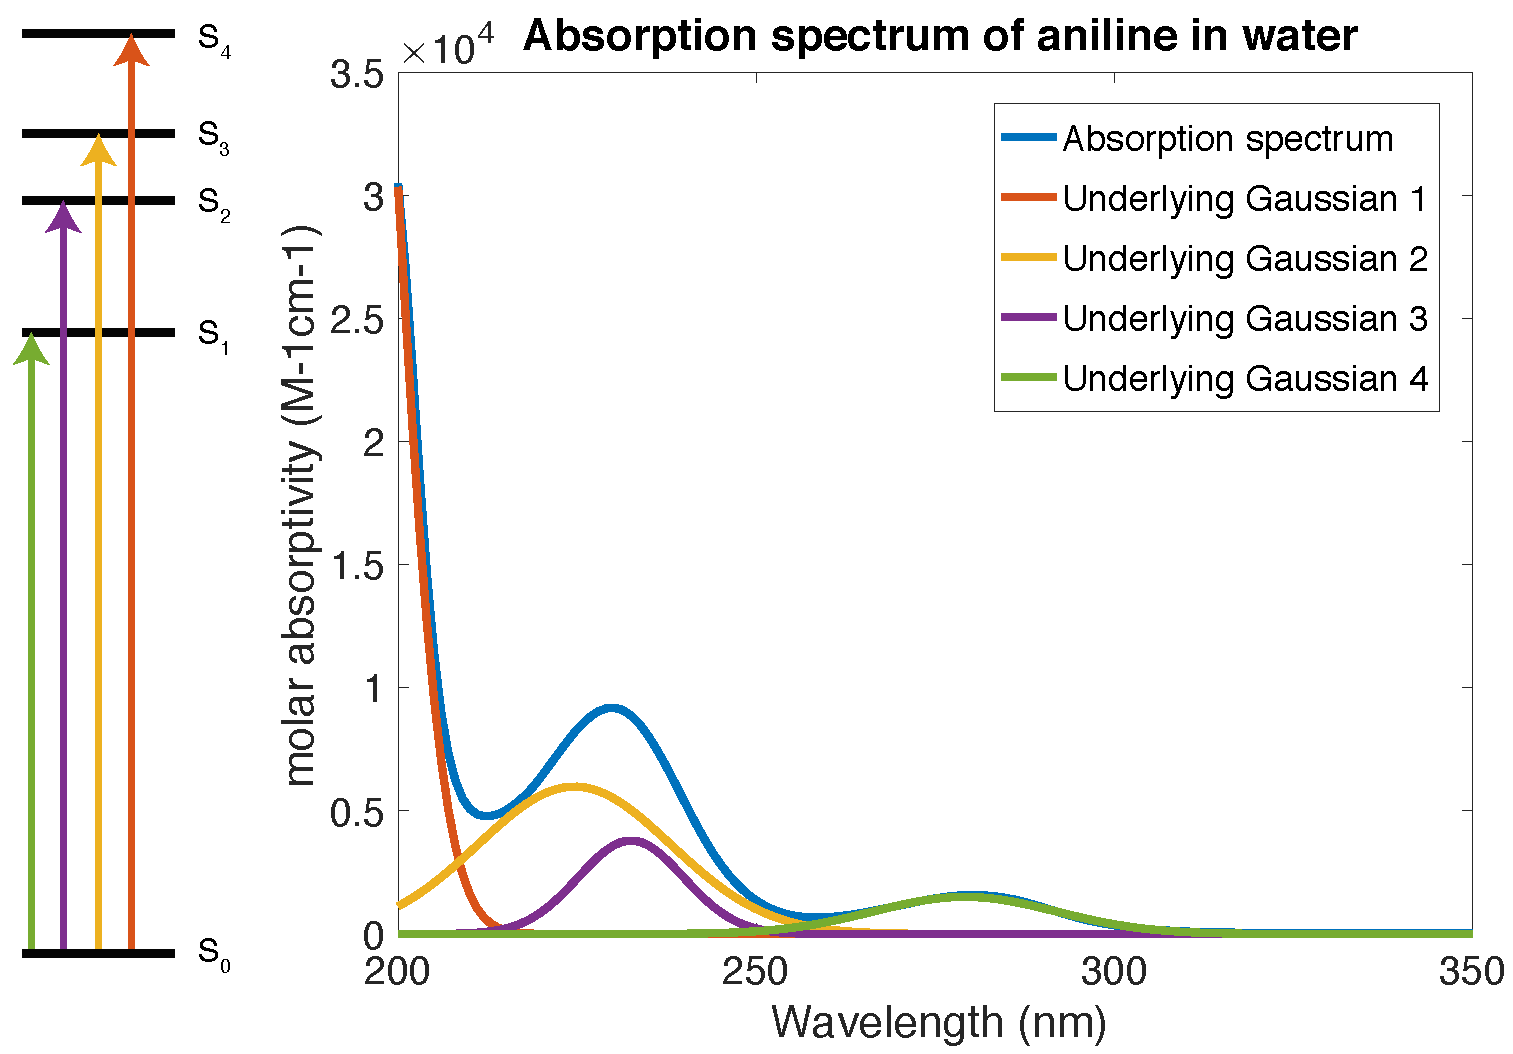
\includegraphics[width=0.48\textwidth]{images/quantum_to_bulk.pdf}
			\caption{Absorption spectrum of aniline in water showing underlying electronic transitions. Underlying Gaussian components, fitted manually using Fityk, refer to 4 electronic transitions as shown in electronic transition diagram on the left. Each peak can be used to calculate oscillator strength using equation \ref{eq:oscillatorStrength}}\label{fig:UVFromFityk}
			\vspace{-30pt}
		\end{wrapfigure}
		
	Secondly, dipole moments from the solvent stabilize the ground state geometry lowering the potential energy surface. Since electrons move significantly faster than the nucleus, excited state geometries are less likely to be stabilized. Unequal lowering of the two potential energy surfaces causes blueshift in excited state energy prediction (see Figure \ref{fig:PESb)}). In gas phase, simulation of UV-VIS spectrum can be done more easily due to a lack of solvent shift and solvent broadening. In solution, sharp and high-intensity gas-phase peaks become broadened and blueshifted. 
	Each individual absorption peak of an electronic transition over a period of wavelength may overlap. A molar absorptivity vs excitation energy plot is a linear combination of normal distribution plots from different electronic transition in a compound. Each individual peak combines together into a continuous experimental spectrum as seen in Figure \ref{fig:UVFromFityk}. Notice different peak width at different excitation modes. Broadening effects from ground state geometry fluctuation affects their excited states differently. 
	Once molecules are excited, solute molecules exist in the high energy state for a period of time. During that time a molecule can undergo different changes: undergoing a reaction by itself, emitting fluorescence light, or relaxing non-radiatively and de-energize back to the ground state. The rate constant of a reaction by the excited state (k\textsubscript{rxn}) and the rate of photon absorption (k\textsubscript{abs}) can determine the likelihood of a certain reaction to occur with respect to the amount of photons absorbed. A quantum yield (\textPhi)for a photo-reaction can then be calculated using Equation \ref{eq:quantumYield}:
	\begin{equation}
	\label{eq:quantumYield}
	\Phi = \frac{\#\ of\ molecules\ undergoing\ a\ reaction}{\#\ of\ photons\ absorbed}=\frac{k_{rxn}}{k_{abs}}
	\end{equation}
	Two main components needs to be determined to evaluate the quantum yield: the reaction rate constant and the light absorption rate constant. Reaction rate can be determined computationally from calculating two potential energy surfaces of the reactant and the product and solving for the conical intersection, where the two surfaces meet.
	
	\begin{wrapfigure}{r}{0.5\textwidth}
		\vspace{-20pt}
		\centering
		\adjincludegraphics[width=0.48\textwidth, trim={{.03\width} {.02\height} {.02\width} {.05\height}},clip=true]{images/4MeOacetophenone_sunlight.pdf}
		\caption{Overlap between absorption spectrum of 4-MeOacetophenone and solar radiation (ASTM G173) showing at which wavelength photons from sunlight can be absorbed to energize the molecule to the excited states. }\label{fig:4MeOOverlap}
		\vspace{-20pt}
	\end{wrapfigure}
	In Eustis lab, Nathan D. Ricke '14 worked on applying computational model to estimate quantum yields of photo-excited small organic molecules in the singlet excited states undergoing Intersystem Crossing (IC) from to the first triplet excited state using Landau-Zener model and outlining a possible method using Fermi's golden rule.\cite{Ricke2014} Landau-Zener model calculates the probability of IC using spin-orbit coupling constant at minimum crossing geometry, energy gradient, and crossing velocity. The rate is then calculated from probability from Arrhenius equation with activation energy being the energy difference between the singlet excited state energy and the conical intersection. Quantum yields of aniline and benzene calculated using this theory were compared with the experimental values. Qualitative agreement with the experiments were observed and discussed. An alternative method is Fermi's golden rule, which calculates rates of transition from one energy state to another from electronic couplings, Franck-Condon factors, and solvent broadening factor. However, the calculation could not be done due to memory shortage caused by the number of terms generated at higher vibrational excitations. Nevertheless, Landau-Zener model can be used to calculate k\textsubscript{rxn} of IC, the numerator term in Equation \ref{eq:quantumYield}.
	
	Since reactions of micropollutants in aquatic environment are the focus of this study, the main photon source for the photo-reactions is the sun. Sunlight at different wavelengths goes through the ozone layer, but most light in the UV range is absorbed by the ozone layer.\cite{Leifer1988} Some of the remaining light photons pass through the atmosphere before hitting the earth surface at a 90 degree. Some disperse in the atmosphere (commonly referred to as sky radiation\cite{Schwarzenbach2005}) before hitting the earth surface at different angles. Light intensity in terms of Solar irradiance (W) can be measured experimentally or looked up on a reference table: ASTM G173-03 Reference Spectra based on conditions considered average in most states in the US and tilt angle representative of the contiguous US states.\cite{astm}   In water body, photon intensity decreases as a function of water depth and its attenuation characterized by the beam attenuation coefficient (\textalpha) and depth (z), both measured experimentally. These physical quantities of sunlight can be combined with the molar absorptivity (\textepsilon) of a species in water to give rate of light absorption (k\textsubscript{abs}) defined by Equation \ref{eq:rateOfAbsorption}:
	\begin{equation}
	\label{eq:rateOfAbsorption}
	k_{abs}(\lambda)=\frac{W(\lambda)\cdot \varepsilon(\lambda)}{z\cdot\alpha(\lambda)}
	\end{equation}
	The focus of this study is to calculate molar absorptivity or equivalent in order to calculate the photon absorption rate in the aquatic environment. Study of UV-VIS absorption processes combined with the two methods outlined by Nathan Ricke illustrate what further calculations can be done to predict the quantum yield of sunlight-driven pollutant degradation in water.	
	
	\subsection{Computational Approach}
	In  recent years, high performance computers have become more and more accessible to researchers.\cite{Dykstra2011} The power of High Performance Computing (HPC) extends the frontier of rigorous computational calculations to solve problems which a decade before were prohibited by the high computational cost (time and resources). To put "high cost" in perspective, wall clock time required to optimize geometry and vibration states of aniline in gas phase using different theories are shown in table \ref{Table:comparisionTheories}. Computational time in the table was generated to provide guidance to understanding computation cost barrier faced when using higher-level theories. Theories are sorted in order of increasing computational time. Due to its accuracy, double excitation Coupled Cluster (CCSD)\cite{Bartlett1978,Pople1978} is considered the hallmark of computational chemistry. Unfortunately, computational time required for CCSD limits its application to only 10-20 molecules; optimization of 14-atom aniline requires 15 computational days. Compared with normal Hartree Fock, CCSD takes 2000 times longer. For larger systems, CCSD becomes impossible to be implemented. With larger number of CPU and more efficient CPU, wall clock time can be faster than computational time. 
	\begin{table}[ht]
		\centering
		\caption{Comparing time required to optimize aniline's geometry and vibrational states and ground state energy using Hartree Fock (HF), DFT, MP2, and CCSD level theory in Gaussian '09\cite{gaussian} to demonstrate how computational time and accuracy varies with different theories. All calculation were done using 6-31G(d) basis sets on a 32-processor node and 10 GB connection.}\label{Table:comparisionTheories}
		\centering
		\begin{tabular}{lllll}
			Theory   & Scaling factor    & Time     &  Time if basis sets double in size   \\ [0.5ex]
			\hline\hline
			\\[-0.5ex]
			HF	&	N\textsuperscript{4} & 10 mins	& 2.7 hours   \\
			DFT & N\textsuperscript{3} & 20 mins	& 2.7 hours  \\
			MP2 & N\textsuperscript{5} & 1 hours  & 32 hours  \\
			CCSD & N\textsuperscript{6} & 15 days & 2.6 years	 \\
		\end{tabular}
	\end{table}
	If basis sets size doubles, the time required can be calculated from the scaling factor (the last column in Table \ref{Table:comparisionTheories}). It becomes clear that CCSD cannot be used for any calculation in a large system. None of the theories here scale linearly, which should reflect certain difficulties when the system becomes larger. MP2 also starts to take longer compared with HF or DFT. 
	\begin{wrapfigure}{r}{0.5\textwidth}
		\vspace{-20pt}
		\centering
		\adjincludegraphics[width=0.48\textwidth, trim={{.03\width} {.02\height} {.02\width} {.01\height}},clip=true]{images/bench.pdf}
		\caption{Visualization of table \ref{Table:benchmarkBasisSets}. Due to their low computational costs compared with CCSD, time values of the other three theories are plotted in a box on the left hand corner. }\label{fig:bench}
		\vspace{-10pt}
	\end{wrapfigure}
	Computational chemists can now implement more rigorous ab initio (from the first principles) methods. As more difficult problems are explored, there is a trend to incorporate both experimental and theoretical methods together for analysis because they have different advantages and disadvantages. For example when studying the photo-degradation of micropollutants, computational approach allows for a priori prediction of photo-products and their impact on the environment. Experimental approach is more limited to a posteriori study of negative impact micropollutants have on water system. Experimental chemists face challenges to study individual species of micropollutants due to complex experiment planning. In natural waters, many species of micropollutants interfere with each other setting limits on what can be measured experimentally in a complex natural system. Experimental methods excel when used to study an observable natural phenomena and its consequences. While theoretical methods are great for studying simple system with good accuracy, they have gained attentions from scientists just in the past decades thanks to burgeoning of growth in computating speed. The computational theories are still in a stage of development as more and more researchers have more access to faster computers. They have become very accurate at calculating small and simple systems. However, ab initio theories remain incomplete and inaccurate for larger and more complex systems. There is still a significant trade-off between cost and accuracy; the question is how much accuracy is needed? There are many factors that increase accuracy and computational cost: Theories, basis sets, solvent models... 
	\begin{figure}[htb]
		\vspace{-10pt}
		\centering		
		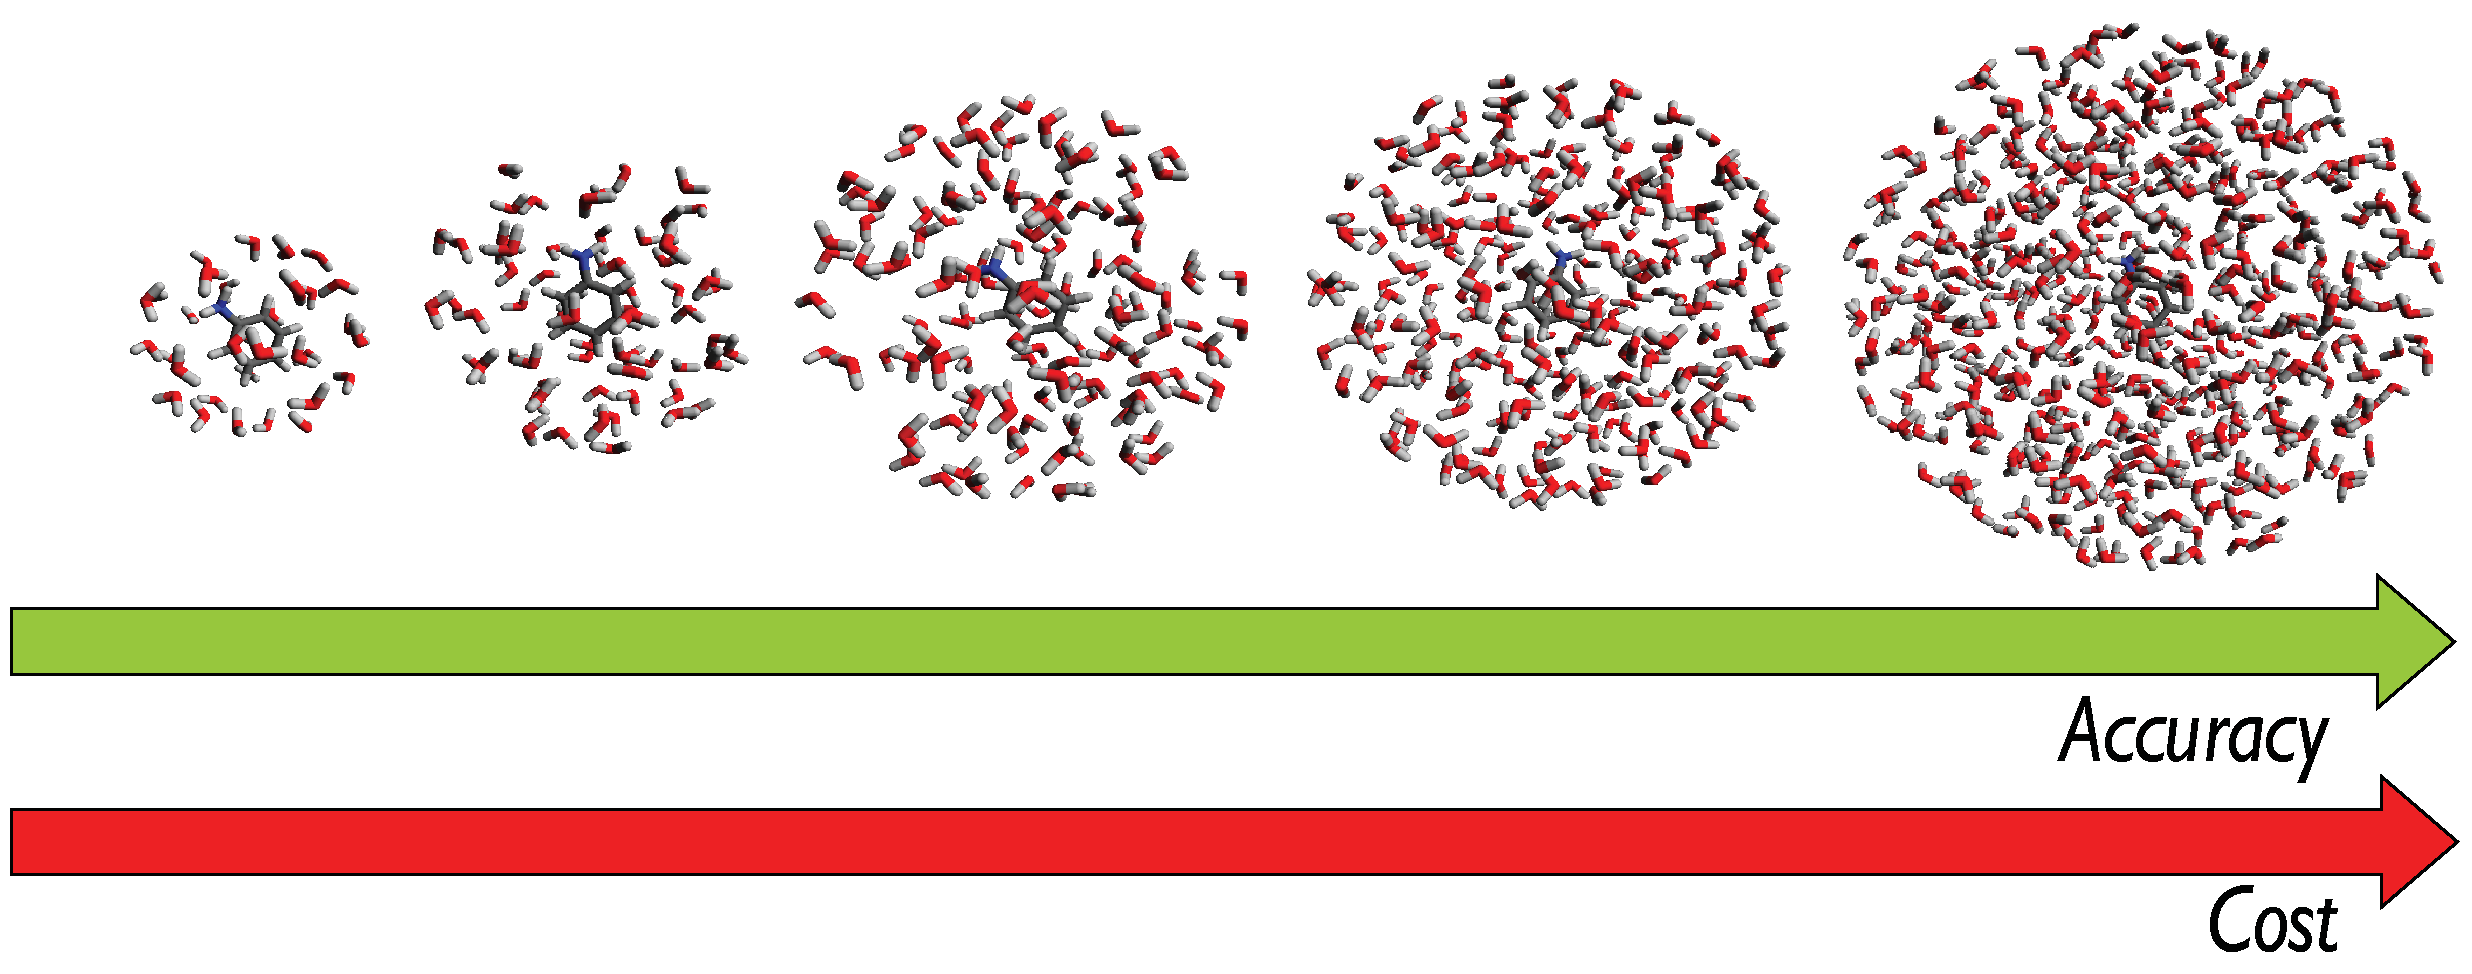
\includegraphics[width=1\textwidth]{images/tradeOff.pdf}
		\caption{ Explicit 2\textsuperscript{n} water model (n = 5-9). The more water, the more complete solute-solvent model but the slower the calculation.}
		\label{fig:tradeOffNumberOfWaterMolecules}
	\end{figure}
	
	The objective of this project is to find a computational model with the best trade of between accuracy and computational cost to simulate excited states energy and probability of excitation of small organic molecules in water compared with experimental results. A work procedure will be developed to systematically evaluate the accuracy of different models. If successful, this procedure will be applicable to other larger molecules of different chemical properties. Criteria of being the best model include good accuracy when compared with the experimental data, reasonable computational cost, and applicability to different models. The best model to calculate the excited states will lead to rate constants of photon absorption, quantum yields, and general prediction of photo-transformation pathways of small organic pollutants.

	\pagebreak
	\section{Background}
	\subsection{Hartree-Fock Theory}
	Schr\"odinger equation is an equation describing the relationship between the energy of system (E) and the wave function (\textPsi) of a wave-particle. It is written in time-independent form:
	\begin{equation}
	\label{eq:schro1}
	H\Psi=E\Psi
	\end{equation}
	\begin{equation}
	\label{eq:schro2}
	H = -\frac{\hbar^{2}}{2m}\nabla^{2}+V
	\end{equation}
	with \textit{H} is the Hamiltonian operator, which describe what the energy of the system is controlled, written here in italics instead of with a circumflex mark over the operator (in physics and computational chemistry, \textit{H} is the convention more commonly used). The left operator is the kinetic energy operator with Laplace operator written using the del symbol. For simple external potential energy conditions like particle in a box or harmonic oscillator, the wave function can be deduced from the Schr\"odinger equation and its energy calculated. More information about Schr\"odinger equation can be found in any elementary quantum mechanics books.\cite{Eisberg1985,Griffiths2005} For a system with more than two or more electrons, there is no direct way to solve the Schr\"odinger equation for an analytic wave function. Variational principle can be used to find the most "correct" numerical wave function that satisfies an eigenfunction in lieu of the Hamiltonian operator in a certain theories. With a trial wave function (\textit{\straightphi}\textsubscript{trial}), energy calculated from the Hamiltonian operator is always higher than energy calculated using the true wave function (\textit{\textpsi}\textsubscript{real}): 
	\begin{equation}
	\label{eq:LCAO1}
	\left \langle \psi_{real}^{*} | H | \psi_{real}  \right \rangle \leq \left \langle \phi_{trial}^{*} | H | \phi_{trail}  \right \rangle 
	\end{equation}
	According to this principle, one can keep modifying parameters in the trial wave function until the calculated energy converges to the lowest value before concluding that the trial wave function is the best representation of the real wave function. The lowest energy calculated is by no means the "correct" value. Theories make assumptions and those assumptions limit how accurate the lowest energy of a theoretical calculation can achieve. Another useful assumption widely used in quantum chemistry is Linear Combination of Atomic Orbitals (LCAO) which allows \textit{atomic} orbital wave functions (\textchi\textsubscript{n}) to be summed to create a \textit{molecular} wave function (\textit{\straightphi}\textsubscript{i}):
	\begin{equation}
	\label{eq:LCAO2}
	\phi_{i} =a_{i1}\chi_{1}+a_{i2}\chi_{2}+a_{i3}\chi_{3}++a_{i4}\chi_{4}+...
	\end{equation}
	Wave function theories mostly use this assumption. One fundamental theory, on which many other theories are base, in computational chemistry is Hartree-Fock Theory (HF). HF theory make assumptions about wave functions and the nature of quantum mechanical interactions in the atomic systems, including LCAO, single-electron wave functions decoupling, and non-relativistic electrons, to arrive at Fock operator (\textit{F}) for a single-electron wave function:
		\begin{equation}
		\label{eq:Fock}
		F_{i}=h_{i}+\sum_{j}^{N}(J_{i}-K_{j})
		\end{equation}
	with \textit{h} being the kinetic and electron-nucleus Coulomb potential energy of an electron, \textit{J} electron-electron Coulomb interactions, \textit{K} electron-electron exchange (a term for Pauil Exclusion Principle). Eigenvalues of \textit{F} are matrices with Lagrange coefficients. These coefficients can be used to calculate energies of each one-electron wave functions before being added back together to calculate total energy of the system. Iterations of guessing a trial wave function through LCAO coefficient adjustment, operating \textit{F} on each single-electron wave functions, and energy calculations are done until the system with the lowest energy is achieved. Limitations of HF are in its assumptions. First, electrons are coupled so single-electron wave functions cannot truly represent one electron without taking into account electron-electron correlations. One of many post-HF theories, most notably M{\o}ller---Plesset perturbation theory (MP)\cite{Møller1934}, attempts to add electron-correlation to correct errors introduced by approximations in HF. 
	
	\subsection{Basis Sets}
	To describe electron orbitals in a molecule, wave functions for quantum calculations are modeled using mathematical functions called basis sets. Simple Gaussian-type basis sets are a combination of Gaussian distributions modeling different orbitals in Cartesian coordinates. They were designed by John Pople to be optimized for speed.\cite{Hehre1986} Smaller basis sets have fewer basis functions per atom. In addition to having higher functions per atom, larger basis sets may also include polarized and diffuse basis sets. Equation \ref{eq:LCAO2} can be rewritten to include two 1S orbitals of two hydrogen atoms in hydrogen gas:
	\begin{equation}
	\label{eq:basisSet1}
	\phi_{H_{2}} =a_{1}\chi^{1S}_{H_{A}}+a_{2}\chi^{1S}_{H_{B}}
	\end{equation}
	While this wave function is adequate to describe ground state hydrogen gas, it will certainly fail to describe the excited state which requires  orbitals in the second electron shell for the electrons in the excited states. Therefore, more orbitals can be added to better describe the molecular orbitals:
	
	\begin{equation}
	\label{eq:basisSet2}
	\phi_{H_{2}} =a_{1}\chi^{1S}_{H_{A}}+a_{2}\chi^{2S}_{H_{A}}+a_{3}\chi^{2P}_{H_{A}}+a_{4}\chi^{1S}_{H_{B}}+a_{5}\chi^{2S}_{H_{B}}+a_{6}\chi^{2P}_{H_{B}}
	\end{equation}
	The atomic orbitals can also be described by analytical mathematical expressions controlled by numerical parameters like Gaussian distributions. For example, in describing the molecular orbitals in aniline molecule, there are different level Gaussian basis set to choose from: STO-3G, 3-21G, 6-31+G(d), ...,  6-311++G(2d,p).
	\begin{figure}[!tbp]
		\centering
		\begin{subfigure}[b]{0.48\textwidth}
			\adjincludegraphics[width=1\textwidth, trim={{.03\width} {.02\height} {.07\width} {.05\height}},clip=true]{images/STOvSTO3G.pdf}
			\caption{}
			\label{fig:visualizingBasisSetsa)}
		\end{subfigure}
		\hfill
		\begin{subfigure}[b]{0.48\textwidth}
			\adjincludegraphics[width=1\textwidth, trim={{.03\width} {.02\height} {.07\width} {.05\height}},clip=true]{images/probDistPlot.pdf}
			\caption{}
			\label{fig:visualizingBasisSetsb)}
		\end{subfigure}
		\caption{Visualization of basis sets. a)plots of STO and STO-3G with its Gaussian components. All three Gaussian plots with 0.44, 0.54, and 0.15 mixing coefficients are added to STO describe atomic orbitals better. First, there is no more discontinuity in the first derivative of the wave function as in STO. Gaussian functions are also easier to integrate compare with exponential functions. Data replotted with permission from Magalh{\~a}es\cite{Magalhaes2014}. Copyright 2014 American Chemical Society. b) probability density of different atomic orbitals. Diffuse functions can be added to light and heavy atoms to better describe more diffuse orbitals when electrons move further away from the nucleus. In this figure, 2S and 2P can increase the distance an electron wave function describe with expanded probability distribution.}\label{fig:visualizingBasisSets}
	\end{figure}
	STO\cite{Hehre1970} is a Slater-type minimal basis set designed for fast calculation. It is the solution to 1S Hydrogen atom using only an exponential function.  In contrast, STO-3G mixes STO with 3 more Gaussian functions to describe the wave function more accurately (see figure \ref{fig:visualizingBasisSetsa)}). 3-21G is also a small model (cheap and simple). It contains 3 Gaussian functions for inner shell orbitals, 2 and 1 different level of Gaussian functions describing valence electrons. 6-311++(2d,p) is more complete but also more expensive. It contains 6 Gaussian functions for inner shell orbitals, 3, 1, and 1 different level of Gaussian functions describing valence electrons. In addition, ++  means it adds two large s orbitals and one large p orbitals \textit{diffuse} functions. This is important in calculating reactions with electron being further away from the nucleus such as electron addition, electronic transition, or charge transfer. Finally, (2d,p) means heavier atoms also contain two d orbitals polarized to the P orbitals and hydrogen atoms p functions to s orbital. Polarized basis sets becomes important when describing physical properties involving electron excitations. 
	
	Another one of the most well-known basis sets is the Dunning's correlation-consistent polarized Core and Valence (Double/Triple...) Zeta (cc-pVXZ) type basis sets. They are basis sets in spherical coordinates that contain variationally optimized coefficients for electron correlations (in contrast to Pople's which was optimized for Hartree Fock). Dunning's cc-pVXZ basis sets may include a large number of polarized basis sets based on what level of Zeta is used. For example, cc-pV6Z describes a second-row atom using 140 basis sets.\cite{Cramer2005} Diffuse basis sets can be added to cc-pVXZ with aug- keyword in front of the basis sets. In comparing among theoretical calculation, aug-cc-pVQZ (ACCQ) can be used as theoretical benchmark.\cite{Rohrdanz2008,Barnes2014} ACCQ's computational cost is however prohibitive for solute-solvent model with Bowdoin HPC. 
	\begin{table}[ht]
		\centering
		\caption{Demonstrating how time required to optimize hydrogen gas geometry and vibrational states and ground state energy using different basis sets in Gaussian '09. All calculation were done with HF level of theory on a 24-processor node and 64 GB of RAM. This table underscores trade-off between accuracy and cost using aug-cc-pvQz as the theoretical benchmark}\label{Table:benchmarkBasisSets}
		\centering
		\begin{tabular}{llll}
			Basis Set	&	Time (seconds)	&	Energy (Eh)	&	R (A) \\ [0.5ex]
			\hline\hline
			\\[-0.5ex]
			3-21G	&	134	&	-1.1230	&	0.735 \\
			6-31G	&	133	&	-1.1268	&	0.730 \\
			6-311G	&	137	&	-1.1280	&	0.732 \\
			6-31G(d,p)	&	154	&	-1.1313	&	0.732 \\
			6-311G(d,p)	&	153	&	-1.1325	&	0.735 \\
			6-311G(d,2p)	&	163	&	-1.1330	&	0.734 \\
			6-311G(d,3p)	&	161	&	-1.1331	&	0.734 \\
			6-311G(d,3pd)	&	194	&	-1.1331	&	0.734 \\
			aug-cc-pvQz	&	3250	&	-1.1335	&	0.734 \\
		\end{tabular}
	\end{table}
	
	To put computational time required by different basis sets in perspective, hydrogen gas geometry can be optimized using different Gaussian-type basis sets and aug-cc-pv6z. This computational demonstration illustrates the main points addressed below about how size of different basis sets affect time and accuracy. As basis sets size increased, computational time increased and energy converged closer and closer to that of the theoretical benchmark.  6-311G(d,2p) is the best basis sets for geometry optimization because it used 20\% less time to calculate compared with 6-311G(2d,p), but with the same degree of accuracy. It is worth noting that depending on the type of calculations and the size of the systems, different basis sets should be chosen to best balance accuracy and cost.
	Adding (d,p) polarized basis sets helped get more accurate H-H radius both in 6-31G to 6-31G(d,p) and 6-311G to 6-311G(d,p). However, within Gaussian-type basis sets group, changes in time as more basis sets added was not as drastic as moving from 6-311G(d,3pd) to ACCQ which takes 15 times longer time to run. When the system becomes larger, the calculation time scaled would become longer. Increasing the size did not always increased accuracy. Note that the radius calculated using 6-311G(d,p) converged to 0.734 Angstroms, close to theoretical benchmark at 0.735 Angstroms. Increasing the size of the basis sets after did very little to improve the value. Different types of calculation then would be more suitable with different basis sets: 6-311G(d,p) for geometry optimization and 6-311G(d,2p) for energy calculation. In calculating excited state energies of organic molecules\cite{Wiberg2004,Barnes2014}, while having cheaper cost, an average-sized basis set 6-311++G(2d,p)\cite{Feller1996} performs better than aug-cc-pVDZ (ACCD)\cite{Feller1996}. For example, transition energies calculated of CN molecule as calculated by ACCD deviates 1117-1669 cm\textsuperscript{-1} from experimental value while those by 6-311++G(2d,p) only deviate 220-470 cm\textsuperscript{-1}.\cite{Barnes2014}
	
	\subsection{Density Functional Theory}
	In theory, Density Functional Theory (DFT) does not require making assumptions about electron-electron decoupling because it does not encounter problems with degrees of freedom as wave-function-based methods do. It therefore has potential to be more exact  compared to HF or post-HF wave function methods. Despite its low costs, DFT's accuracy in certain applications has been accepted and acclaimed.\cite{Baerends1997,Sousa2007}	Wave-function-based methods locate each particles in wave functions with 3 parameters on cartesian coordinates.
	\begin{equation}
	\label{eq:psi}
	\Psi (x_{1}, y_{1}, z_{1}, x_{2}, y_{2}...)
	\end{equation}
	In multi-particle systems, computational cost rises exponentially with the number of particles. For a large solute-solvent system, the calculation cost becomes expensive. DFT uses electron density function with only 3 Cartesian parameters. Despite having fewer parameters, density functions also contain data about total number of electrons, position of nuclei, and atomic number; all required to calculate the Hamiltonian operator.
	\begin{equation}
	\label{eq:rho}
	\rho (x, y, z)
	\end{equation}
	Energy of a density function is not calculated based on HF or other wave function methods. Historically, DFT had large errors and limited usage in computational chemistry because there is no analytical or numerical way to solve for electron density functions. In wave function based methods, variational principles governs that energy calculated from the operating Hamiltonian on a candidate wave function gives higher energy than on the correct wave functions. By adjusting the wave function, until its energy is minimized, a wave function as a solution to that Hamiltonian operator can be solved for numerically. Two important theorems developed by Pierre Hohenberg and Walter Kohn allow DFT to be used more broadly in computational chemistry community by providing a way to calculate the energy via variational principle.\cite{Hohenberg1964} The first theorem states that only ground state electron density is required to construct the external potential function and hence the Hamiltonian. This is important because potential for excited state wave functions can also be calculated. The second theorem, is the variational principle for DFT allowing to change parameters in the density function to get lowest energy through wave function and Hamiltonian calculation.
	\begin{equation}
	\label{eq:HK2}
	\left  \langle \Psi_{cand (DFT)}^{*} \left | H \right | \Psi_{cand (DFT)} \right \rangle = E_{cand (DFT)}\geq E_{0} 
	\end{equation}
	The problem with DFT as described is variational principle calculation on the wave functions because it requires solving the Schr\"odinger's equation to obtain the wave function and make assumptions/approximations as discussed above. To solve this, Kohn-Sham Self-consistent Field (Kohn-Shan SCF), developed in 1965, made use of the two theorems by breaking down electron density to non-interacting single-electron density functions.\cite{Kohn1965} Energy functionals can then operate on linear combination of these electron functionals to give the energy of the system. Functionals are functions which operate on another function. Instead of using the Hamiltonian operator and a wave function to calculate the energy (Equation \ref{eq:schro1}), Kohn-Shan SCF calculates the energy of the system directly from electron density function using different functionals. For example, the Kohn-Sham one-electron operator as presented in Cramer's Essentials of Computational Chemistry\cite{Cramer2005}: 
	\begin{equation}
	\label{eq:KSH}
	h_{i}^{KS}=-\frac{1}{2}\nabla_{i}^{2}-\sum_{k}^{Nuclei}\frac{Z_{k}}{\left | r_{i}-r' \right |}+\int \frac{\rho(r')}{\left | r_{i}-r' \right |}dr' +V_{xc}
	\end{equation}
	with the familiar looking first two terms (see Equation \ref{eq:schro2}). The last term on the right hand side of the equation refers to exchange-correlation functional; it includes quantum mechanical exchange, electron correlation, and correction in kinetic and potential terms. Exchange interaction in fermions like electrons follows Pauil Exclusion Principle, constraining electrons from being described by the same quantum numbers. Correlation is an electron-electron interaction term ignored in HF. In modern DFT functionals, experimentally fitted parameters are used to describe these energy functional components.\cite{Cramer2005} Different functionals have different fitted parameters and their accuracy dependent on the system and physical properties being calculated. To find the best group of functionals for calculating excited state energies, there needs to be a benchmark specifically on excited state energy calculation on similar systems and electronic states. In modern functionals, a functional of electron density gradient function is added to the energy functionals.These functionals are gradient corrected and the method called generalized gradient approximation (GGA). Pure GGA functionals is known to underestimate system energy\cite{Heßelmann2015,Hirao2011, Parac2002, Jacquemin2009} or excited state energy\cite{Caricato2010, Barnes2014}.  In addition, a percent of contribution calculated from HF can be mixed in with the pure GGA results to create GGA-HF hybrid functionals. According to Hellmann-Feynman theorem (Equation \ref{eq:xc1}), an actual exchange-correlation energy can be described as an energy plot over extent of correlation (\textlambda), as shown with green shaded area in Figure \ref{fig:xcDFT} recreated here based on figures in two literature sources.\cite{Cramer2005, Bersier} Area of box A and B respectively refers to pure HF exchange energy and pure GGA exchange-correlation energy. Since the energy as a function of extent of correlation is not known, experimentally fitted value (z) is needed to find the integral using Equation \ref{eq:xc2}. Adding HF exchange energy reduces overestimation of energy calculated from GGA functionals.
	\begin{equation}
	\label{eq:xc1}
	E_{xc}=E_{xc}=\int_{0}^{1}\left \langle \Psi (\lambda)\left | V_{xc} \right | \Psi (\lambda)\right \rangle d\lambda
	\end{equation}
	\begin{equation}
	\label{eq:xc2}
	E_{xc}=E_{x}^{HF}+z(E_{xc}^{GGA}-E_{x}^{HF})
	\end{equation}
	\begin{wrapfigure}{r}{0.5\textwidth}
		\vspace{-10pt}
		\centering
		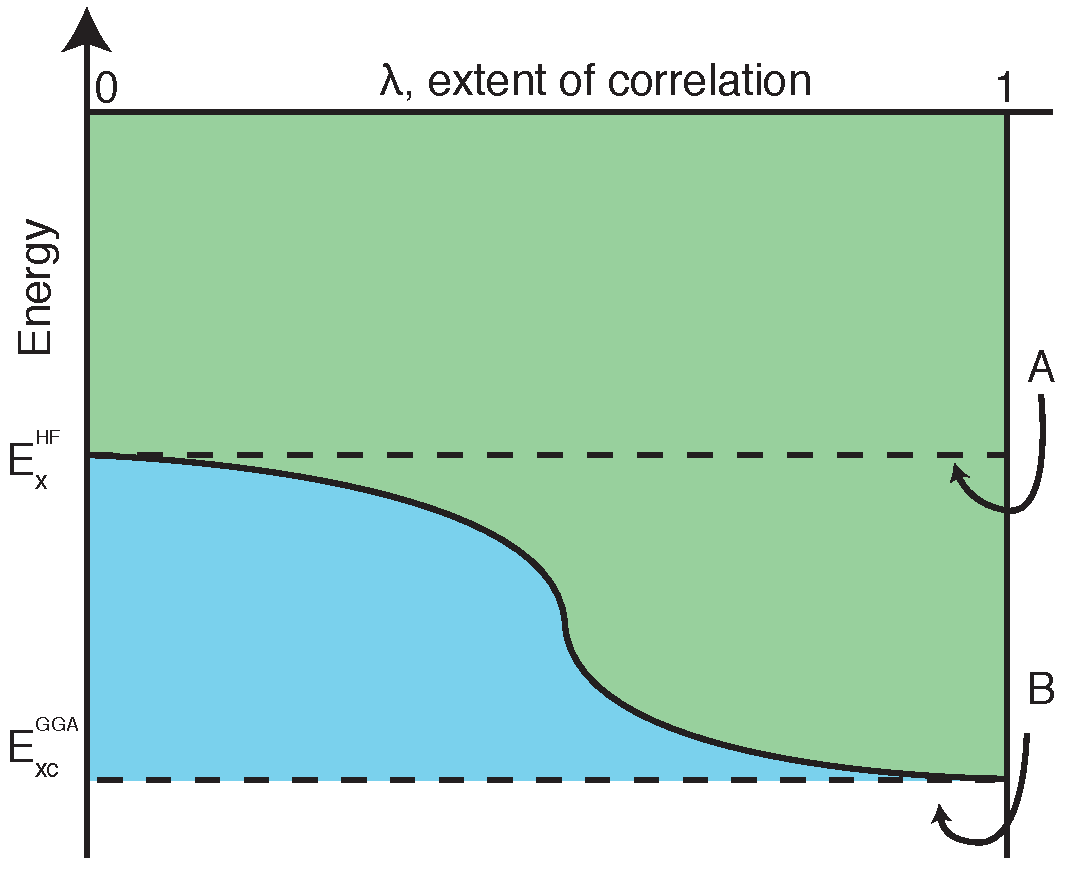
\includegraphics[width=0.48\textwidth]{images/xcDFT.pdf}
		\caption{Illustration of hybrid exchange-correlation term from HF and DFTrecreated here based on figures in two literature sources.\cite{Cramer2005, Bersier}. Box A drawn by the first dotted line is an integral of exchange-only energy calculated from HF from \textlambda value 0 to 1. Box B drawn by the second dotted line is the same integral but of exchange-correlation energy calculated from pure-GGA DFT. The value of actual exchange-correlation energy (shaded green) is likely to be described by the value between area of box A and B.}\label{fig:xcDFT}
		\vspace{-15pt}
	\end{wrapfigure}
	Functionals with HF component are called hybrid functionals.  Some of the more widely-used hybrid functionals include: B3LYP, CAM-B3LYP\cite{Yanai2004}, M06-2X\cite{Zhao2007}, and PBE0\cite{Adamo1999}. New functionals can also be created from mixing one functional for exchange and one for correlation. For example, BP86 is a combination of B88 for exchange and P86 for correlation. Unlike basis sets, which can become more complete as number of basis sets per atom increases, there is no 'full,' or complete, functional to use. 
	Among all current theories to calculate the excited states, Time-Dependent Density Functional Theory (TD-DFT) is the most promising with its high accuracy when used with appropriate functionals and low computational cost\cite{Magyar2007}. TD-DFT calculate the electron density response to excitation photon modeled as an external perturbing field varying with time.\cite{Runge1984}  Despite its under-performance in certain systems like organic dyes\cite{Caricato2004} and sulfur organic compounds\cite{Fabian2001}, studies suggest limitations can be overcome if appropriate funcitonals are used.\cite{Barone2007a, Jacquemin2009}  According to one study of 0-0 transition in radicals, the two best-performing DFT functionals are CAM-B3LYP and M06-2X. Pure GGA functional BP86\cite{Becke1988,Perdew1986} and long range corrected GGA  LCBLYP\cite{Iikura2001,Lee1988,Becke1988} are also attractive to have a diverse group of functionals.
	
	\subsection{Solvent Models}
	Despite the recent advent of growth in computer speed and the burgeoning interest in incorporating computational models to further understand the natural world, large systems such as solvation models remain a big challenge.\cite{Lin2007} In describing the solvents, one can either apply bulk solvent effect on the solute through different potentials without specifying the solvent molecules (implicit solvent model) or one can explicitly place the solvent molecules around the solute molecule (explicit solvent model). When calculating excited states energy of a solute, solute-solvent interactions will contribute to modeling solvent effects on absorption spectra as previously discussed  (Figure \ref{fig:PESa)} and \ref{fig:PESb)}). In the past, implicit solvation models were frequently implemented because they gave acceptable results while maintains low computational cost. In contrast to explicit model, interactions between each individual solvent molecule and the solute molecule are not calculated. The most commonly used implicit model is the Polarizable Continuum Model (PCM).\cite{Cossi2000, Mennucci2010, Tomasi2005} Instead of explicitly handling each solvent molecule quantum mechanically, PCM expresses their bulk effects on solute molecule in means of dielectric continuum field surrounding molecule of interest. Dielectric field can polarize and affect the wave function of the solute system. Its disadvantage is its lack of dynamic solvent contribution on excited states properties.\cite{Barone2007a} Implicit solvent models also neglect hydrogen-bonding as they assume implicit implementation in dispersion forces and electrostatics.\cite{Li1999} In molecules with hydrogen bonding, implicit solvent model fail at quantum mechanical level to fully model solute-solvent interactions. Having more rigorous calculations, explicit solvent models, require more computational cost compared with implicit water models. Cost for treating a solute molecule in a large solvent sphere with full quantum mechanics can become prohibitive depending on basis sets, theory, the number of explicit solvent molecules (see Table \ref{Table:comparisionTheories} and Figure \ref{fig:tradeOffNumberOfWaterMolecules}). One recent notable model, Effective Fragment Potentials (EFP), can be used to model explicit solvent molecules with non-bonded van der Waals interactions, hydrogen bonding. It implements Coulomb interactions, polarization, and exchange repulsion without high computational expense of explicit models.\cite{Day1996,Yoo2008} Implementing EFP solvent model, TD-DFT can be used to accurately calculate excited state energy of acetone in water.\cite{Yoo2008} In incorporating the solvent model, there are also two different methods: static or dynamics. In static model, geometry optimization of solute molecule is carried out, then followed by calculation of excited state energies. This static ground state molecule however does not accurately represent solute in water.\cite{Defusco2011} As discussed earlier, the system molecules are dynamic. The difference in solute geometries can broaden the solute's excited state energies in solvent. Instead, Molecular Dynamics (MD) of solute and EFP solvent fragments can be used to obtain a range of equilibrated structures at a specific temperature (see Figure \ref{fig:MDdataa)}). Mark Gordon et al. averaged the calculated energies of each excited state to arrive at a final excited states energy.\cite{Defusco2011}
		
	\subsection{Molecular Dynamics}
	Canonical Ensemble Molecular Dynamics (NVT)\cite{Schmidt1993} provides a pool of equilibrated ground state geometries under constant number of particles, volume, and  room temperature, 298K (see Appendix). Starting with a higher-energy initial geometry, a system relaxes to lower potential energy state until it reaches the dynamic equilibrium. However, there is no accepted measure of equilibrium. One study by Chodera suggests looking at how density of liquid argon changes over time and using variance-bias trade off to find equilibrium period.\cite{Chodera2015} By eliminating non-equilibrated geometries, the rest of the equilibrated geometries become "equilibrated" samples. As requirements for the equilibrium determination are relaxed, more "equilibrated" samples can be used for further calculations, the variance of the value calculated decreases. However, error from including non-equilibrated geometries (bias) increases as more samples, which has not really reached the equilibrium enter the pool. The best trade-off were determined to be a cut off-time when the ratio of sampling size to estimated statistical inefficiency is maximized. For a large system like organic solvent-solute model, this algorithm cuts off too much of the sampling size so it follows that its estimate of statistical inefficiency is not accurate. According to the study, the accuracy of cut-off should be questioned if the whole sample time is not at least an order of magnitude larger than cut-off time value.
		
	\subsection{Comparing Experimental And Theoretical Calculation Results}
	As discussed above, experimental molar absorptivity is not a characteristic of a chemical property; the value depends on solvent broadening and measurement resolution. Molar absorptivity at a single wavelength value(\textepsilon, M\textsuperscript{-1}cm\textsuperscript{-1}), with a value range of 0 to 50000 M\textsuperscript{-1}cm\textsuperscript{-1}, may qualitatively imply probability of transition. The larger the molar absorptivity, the larger the absorptivity, the more photons absorbed. Molar absorptivity does not have an upper limit. Results obtained from theoretical calculations are composed of excited states energy (E, nm) and oscillator strength (no unit).\cite{Hilborn1982} Oscillator strength, with range from 0 to 1, is a measure of how probable a specific electronic transition can occur. There is no solvent broadening involved in calculating static oscillator strength from a geometry, therefore theoretical oscillator strength cannot be compared with molar absorptivity directly.  Oscillator strength tells the degree of allowness of transition between two electronic states. Mathematically, oscillator strength can be calculated from integrating molar absorptivity over a range of wavenumber within an electronic transition (see equation \ref{eq:oscillatorStrength}).\cite{Klan2009}
	\begin{equation}
	\label{eq:oscillatorStrength}
	f = 4.3\times 10^{-9}\int_{\widetilde{\nu}_{a}}^{\widetilde{\nu}_{b}}\varepsilon(\widetilde{\nu}) d\widetilde{\nu}
	\end{equation}	
	
	\clearpage
	
	\section{Methods}
	\subsection{Overview} \label{step1}
	Systematic approach to developing computational model is outlined in this section. Python\cite{python} scripts were used to facilitate some of the steps (see Appendix). Aniline was chosen as the initial test solute due to its hydrogen bonding capability, its small size, and extensive previous experimental and theoretical work on aniline within the Eustis lab. A successful model of aniline was expected to be applicable even to larger molecules of similar class, organic and aromatic. Starting molecule geometries were obtained from optimizing the molecular geometry of the solute and solvent molecules yielding two optimized geometries for solvent and solute. These two geometry files were then inputed into Packmol program\cite{Martinez2009} with empirical guess initial solvent radius and number of water molecules to create starting geometry of solvated solute. MD-TD-DFT using the geometry from Packmol was performed using GAMESS quantum computational package. All MD run used 6-311++G(2d,p) basis sets, calculating velocity vector every 1 fs while calculating other physical properties displaying every 10 fs at bath temp = 298 K. All TD-DFT calculations use 6-31+G(d,p) basis set. Water molecules were modeled explicitly using EFP1 and positioned initially using Packmol. Criterion for MD equilibrium is that the average change of system’s potential energy over time crosses zero. After equilibrium has been reached, a 10 ps of equilibrated geometries are used in calculating excited state energies using TD-DFT in GAMESS. Matlab\cite{matlab} was used to deconvolute experimental spectra and theoretical data cluster.
	The flowchart for finding the best model is outlined below in Figure \ref{fig:flowchart}. First, the optimal number of water molecules in the model was evaluated by using different numbers of water molecules surrounding aniline with CAM-B3LYP functional. The results were compared with experimental data to evaluate the accuracy of the model. The model which contained the lowest number of water, but still provided the most accurate results compared with experimental data is chosen, then applied to other molecules with different functionals before compared again to experimental data. 
	
	\begin{figure}[!htb]
		\centering		
		\includegraphics{images/flowchart.pdf}
		\caption{Flowchart of work in this project. Python scripts were utilized to facilitate certain steps. Section and page number of important steps are listed here: reason for "Start with aniline in water," Section \ref{step1} on page \pageref{step1}; procedure for "Use CAMB3LYP and 2\textsuperscript{n} water molecules," Section \ref{step2} on page \pageref{step2}; results and discussion of "Run MD" and "Calculate excited state energies using TDDFT" Section \ref{step3} on page \pageref{step3}; "Compare how fast the system equilibrate," Section \ref{step4} on page \pageref{step4}; "Compare with experimental data," Section \ref{step5} on page \pageref{step5};}
		\label{fig:flowchart}
	\end{figure}
	
	\subsection{Computational}
	
	\subsubsection{Facilitating Each Steps Using Python Scripts}
	Python scripts play an important role in both data collection and smoothing the process between each computational steps. In order to automatically generate input files and cultivate output data from output files, many python scripts were written from scratch (see Appendix). Since each script is specific to each calculation task, there is a limited number of scripts available on the internet (virtually none for this project) Log files obtained from GAMESS contains both valuable theoretical data and useless text strings.  For example, even though WebMO\cite{webmo} automatically generates last geometry calculated from MD run, extracting a geometry from each MD step requires one to manually open the log file, copy-paste, reformat each geometry into an input file for TD-DFT calculation one geometry at a time. The python script postMDDataPull2.py is designed to pull thousands of geometries and generate GAMESS input files for TD-DFT energy calculation within seconds. In some cases, using Python scripts was required. When running MD of 512 water molecules, the size of the log file became so large (15 GB). The text files that size are unsupported by any regular graphical interface text editor. Extra care were taken when designing these scripts to deal with large data to make sure fast speed is maintained and results consistent when applied to different files. Generating these python scripts will also allow unified program to be developed in order to automate the whole project without any manual input.
	
	\subsubsection{Preparing Starting Geometry Using Packmol} \label{step2}
	As in many theoretical calculation, an initial guess is required. In MD, initial geometries of the solute and solvent were required to start MD calculations in GAMESS. This guess geometry was calculated using Packmol by inputting optimized geometries of solute and solvent calculated from using DFT with CAM-B3LYP functional and 6-311G(2d,p) basis sets. A sample of Packmol input file for solvating aniline in 16 water molecules is displayed below. The program does not return system geometry unless solvent molecules can fit in smallest, user-specified, radius without exceeding steric strain controlled by tolerance value (line 25). The value, 2.5 Angstrom, controlled the smallest distance atoms need to be far away from each other (line 6). If molecules could fit, solvent radius is increased slightly until a geometry was obtained. Notice this input command asks for spherical solvent sphere, which is convenient to use when implementing SSBP. If periodic boundary condition is to be used, line 25 should be changed to "inside cube 0. 0. 0. 5." with a cube of dimension 5 x 5 x 5 Angstrom\textsuperscript{3}. 
	\inputminted[linenos, breaklines, baselinestretch=1, fontsize=\small]{Perl}{../PACKMOLinp/aniline16.inp}
	
	\subsubsection{Computational Models} 
	Packmol was used to place water molecules around solute molecules to create starting geometry. GAMESS computational chemistry software was used in calculating MD and excited state energies. Fityk program\cite{Wojdyr2010} was used to fit Gaussian under absorption spectrum (Figure \ref{fig:UVFromFityk}), and theoretical data (Figure \ref{fig:MDdatab)}). In order to accurately calculate the excited energies, the 6-311++G(2d,p) basis sets was chosen to run vertical excitation energies on a set of equilibrated geometries. It was decided to reduce the basis set in running MD. A smaller basis set 6-31+G(d)\cite{Feller1996} was used in order to cut computational cost. In MD calculation, diffuse and polarized basis sets are not as important since electrons do not move as much compared with TDDFT where charge transfer occurs when electrons move from HOMO to LUMO. It is an accepted knowledge that smaller basis sets produces as accurate geometry compared with larger basis sets (see also Table \ref{Table:benchmarkBasisSets}). Smaller basis sets also converge more easily giving better accuracy-cost trade off. EFP1 model of water molecules was chosen to implement an explicit solvent model and calculate excited states energies. The appropriate number of water molecules in the model had never been evaluated. Too many number of water molecules require more expensive computational cost. Too few water will not give a full model of solute-solvent interaction. A binary framework was used to test how many water molecules were needed to fully solvate the aniline: 2\textsuperscript{n}, n=5 to 9 (see Figure \ref{fig:tradeOffNumberOfWaterMolecules}). 
	
	After number of solvent molecules suitable to model solute-solvent for photo-excitations in aniline was decided, MD-TD-DFT excited state energies and oscillator strengths were calculated for 3-F-aniline, 4-F-aniline, 3-Cl-aniline, 4-MeOacetophenone, and (1,3)-dimethoxybenzophenone using that model. Once excited state energies for each system were calculated, the results were compared with experimental spectral data to find which functional performed best at calculating MD-TD-DFT excited states energy.  Since CAM-B3LYP is a good functional for calculating ground state energies, equilibrated geometries will be calculated using CAM-B3LYP, and TD-DFT excited states using different functionals. Other functionals are PBE0, M06-2X, BP86, and LCBLYP. Aspreviously discussed, M06-2X was expected to perform well when calculating excited state energies (see Introduction). PBE0 is a generic hybrid functional. BP86 is a pure GGA function (no HF). LCBLYP is a long range corrected functional.
	
	\subsection{Experimental} 
	Experimental absorption spectra of 6 small organic molecules (aniline, 3-F-aniline, 4-F-aniline, 3-Cl-aniline, 4-MeOacetophenone, (1,3)-dimethoxybenzophenone) in pH 7 water was collected by Alex Poblete '17 and Holly Rudel '17 over the summer of 2015. Experimental methods as written in a currently submitted but unpublished article\cite{Eustis2016} is rewritten here in full. The organic analytes were purified via vacuum distillation under 99.998 \% nitrogen atmosphere and/or as described in the literature\cite{Armarego2013}. Stock solutions (1 - 10 mM) were made in purified methanol and stored in amber vials at 4 degrees Celsius. Type I water (AquaSolutions, $ \geq 18\: M\Omega^{1}cm^{-1}) $ was used for all aqueous solutions.  Solutions were buffered at pH 7.0 with 10 mM phosphate buffer.  Quartz glassware (Starna Cells, USA) was used for all spectroscopic measurements. UV-Vis absorption measurements were performed using a dual-beam (sample/blank) Cary 400 spectrometer. The instrument is calibrated for energy accuracy (holmium oxide gel, Starna) and transmittance (Dichromate) on a regular basis.  scanning from 190 - 400 nm at 1 nm increments at a rate of 50 nm per minute.  The slit width was fixed at 1 nm resolution.  Blank solutions were prepared from the same 10 mM phosphate buffered Type I water.  Instrument correction was performed by inclusion of a blank in each concentration series, and via real-time reference subtraction against an additional blank during each measurement. Each analyte series consisted of a blank and five samples in the concentration range of 5 - 100 \textmu M  The concentration range chosen for each analyte was chosen to avoid concentrations approaching the solubility limit and to provide \textepsilon\textsubscript{lambda} values $\leq$ 0.1 absorbance units for the most concentrated sample.  Issues with insolubility at pH 7 / 25 degrees C were avoided by examining available solubility data\cite{Yalkowsky2016}, assuring all stock and working solutions are fully stirred at room temperature before transfer.
	
	\begin{figure}[!htb]
		\centering		
		\includegraphics[width=0.9\textwidth]{images/abs_added.pdf}
		\caption{Experimental UV-VIS spectra of 6 organic molecules measured in pH 7 water and 298K collected by Alex Poblete '17 and Holly Rudel '17 over the summer of 2015. Each spectrum represents the fitted slope of six samples with values of c from 0 to 100μM, with the Y-error bar representing the standard error or 95\% confidence interval.}
		\label{fig:abs_added}
	\end{figure}
	\clearpage
	
	\section{Results And Discussion}

\subsection{Results from MD-TD-DFT} \label{step3}

\begin{figure}[!htb]
	\centering
	\begin{subfigure}[b]{0.49\textwidth}
		\adjincludegraphics[width=1\textwidth, trim={{.03\width} {.02\height} {.07\width} {.01\height}},clip=true]{images/aniline128_energyPlot_edited.pdf}
		\caption{}\label{fig:MDdataa)}
	\end{subfigure}
	\hfill
	\begin{subfigure}[b]{0.49\textwidth}
		\adjincludegraphics[width=1\textwidth, trim={{.03\width} {.02\height} {.07\width} {.01\height}},clip=true]{images/energyOscillatorStrengthPlot.pdf}
		\caption{}\label{fig:MDdatab)}
	\end{subfigure}
	\caption{MD run and excited state data calculated from TDDFT of equilibrated geometries from MD. a) plot of system's potential energy vs time in MD with geometries shown at t=0, 0.2, 1.78, 2.78 ps. System energy and solvent radius decreased very rapidly in the first 0.2 ps, before converging to the equilibrium value. Fluctuation in energy is strong, around 0.1\% but the equilibrium was determined to be from 1.78-2.78 ps (see methods). b) theoretical data from MD-TDDFT calculation using 1000 equilibrium geometries. Roughly five groups of data can be seen here. It would be erroneous however to assume each excited state energy calculated from one geometry comes from the same excitation mode.}
\end{figure}

To explain procedures and methods used to analyzed the results, MD-TD-DFT result using aniline in 128 water molecules using BP86 functionals was used to as an example case. MD's system potential energy as a function of time was plotted here in Figure \ref{fig:MDdataa)}. Starting solute-solvent geometry at 0 picoseconds (ps) was obtained from Packmol program. Within 20 ps, system energy dropped 1\%. Water sphere radius also appeared to have shrunk from its starting geometry. The decrease in solvent radius was expected. Hydrogen bonding and other intermolecular interactions stabilize the system causing system energy to lower to its equilibrium value. After the first 2 ps, system energy decreased, taking time to slowly equilibrate. In this case, 34.5 ps worth of MD was calculated took 9 days on 32-cpu and 10 Gb connection. Chodera's code\cite{Chodera2015} was used to calculate the cut-off time to be at 30 ps. The sample size should be at least one order of magnitude larger than the equilibrated one for the assumption made to estimate statistical efficiency used in the code to hold true. Assuming this cut-off point to be accurate, at least 300 ps of MD data would be obtained before deciding to choose use 30 ps as a cut-off point with confident. Projecting this forward, it would take 3 months to calculate MD run with time span larger enough to determine the equilibrium using Choreda's method. Instead of using Chodera's code, the equilibrium was determined by plotting linear regression slope of system's potential energy over time with an arbitrarily set interval of 10 ps (equilibration period). The consistently low fluctuation indicated the start of equilibrium at 18 ps. Once the system's energy fluctuation reached zero, that interval should be considered at equilibrium. Slope of linear fit for each 10 ps interval starting at time on x-axis was displayed on Figure \ref{fig:slopePlota)}. When equilibration period was changed to 3 ps (Figure \ref{fig:slopePlotb)}), energy slope reached zero earlier compared to 10-ps. The new equilibrium period yields equilibrium to be established at 6 ps instead of 20 ps. However, reducing equilibration period created larger energy slope fluctuation due to smaller sample size. Systematic criteria of measuring the equilibrium should still be properly explored and studied. 

\begin{figure}[tbp]
	\centering
	\label{fig:slopePlot}
	\begin{subfigure}[b]{0.49\textwidth}
		\adjincludegraphics[width=1\textwidth, trim={{.03\width} {.02\height} {.07\width} {.05\height}},clip=true]{images/aniline128_slopePlot10ps.pdf}
		\caption{}
		\label{fig:slopePlota)}
	\end{subfigure}
	\hfill
	\begin{subfigure}[b]{0.49\textwidth}
		\adjincludegraphics[width=1\textwidth, trim={{.03\width} {.02\height} {.07\width} {.05\height}},clip=true]{images/aniline128_slopePlot3ps.pdf}
		\caption{}
		\label{fig:slopePlotb)}
	\end{subfigure}
	\caption{Slope plot of aniline with 128 water BP86 using different equilibrium period. a) 10 ps. b) 3 ps. Notice the higher in slope fluctuation in (b) compared to (a). This is due to smaller sampling size}
\end{figure}

 After MD equilibrium was found in the 1.78 to 2.78 ps region, system geometries of that region were used to calculate excited states using TD-DFT. Five excited energy states and its oscillator strengths from the ground state were calculated and shown in Figure \ref{fig:MDdatab)}. Since pairs of excited state energy and oscillator strength data are collected over a range of equilibrated starting geometries, statistical analysis of raw theoretical data is required. A Matlab code was developed by Soren Eustis using Bayesian probability to fit Gaussian distribution to raw energy-oscillator-strength pair from Figure \ref{fig:MDdatab)} to Figure \ref{fig:bayesiana)}. The number of Gaussian plots fitted ranges from 1-9 in each sub-figure. The accepted number of plots was determined and the excited state energies and oscillator strengths given by Bayesian Information Criteria score. The lower the score of a sub-figure, the better fit. According to Figure \ref{fig:bayesianb)}, 7 Gaussian components fitted to theoretical data was the best. Results of this fit is shown in the next section. 

 Experimental  absorption spectra needed to be deconvoluted into a mixture of Gaussian functions for oscillator strength calculation of each individual electronic transition (see Figure \ref{fig:UVFromFityk}). Subsequently, each individual function was integrated numerically over the entire energy range of the function to give the total transition intensity using Equation \ref{eq:oscillatorStrength}. After calculation of excited state energies and the oscillator strength, computational results were compared with values calculated from experimental UV-VIS spectrum to evaluate accuracy of the models tested. There are currently no studies using full statistical method on quantitative calculation of excited state energies of organic molecule in water. Currently, Matlab code utilizing Bayesian probability as a statistical technique to properly find the Gaussian plots are being developed by professor Soren Eustis from previous work in R\cite{RDevelopmentCoreTeam2008} with Peter Cohen '18. This allows room for a systematic approach to develop an appropriate computational model that would allow for further understanding of aquatic pollutants. In special cases, more information can be extracted from MD energy plot and system geometries. Two example of this will be discussed in the following sections. 

\begin{figure}[!tbp]
	\centering
	\label{fig:aniline4}
	\begin{subfigure}[b]{0.49\textwidth}
		\adjincludegraphics[width=1\textwidth, trim={{.03\width} {.02\height} {.07\width} {.05\height}},clip=true]{images/differentGaussians.pdf}
		\caption{}
		\label{fig:bayesiana)}
	\end{subfigure}
	\hfill
	\begin{subfigure}[b]{0.49\textwidth}
		\adjincludegraphics[width=1\textwidth]{images/BICplot.pdf}
		\caption{}
		\label{fig:bayesianb)}
	\end{subfigure}
	\caption{ Results from Bayesian analysis using a Matlab code developed by Soren Eustis. a) deconvoluted theoretical excited state energies (E, eV) and oscillator strength (f, unitless) with varying number of Gaussian components from 1 to 9. Notice even after 5 apparent clusters were plotted, more Gaussian functions were can still be added. b) Bayesian information criteria score as a function of increasing number of fitted Gaussian functions. The lower the score, the better the fit. In this particular plot, the best number of Gaussian plots is 7.}
\end{figure}

	\subsubsection{Solvent Boundary Potential}
	At room temperature, volatile solvent molecules like water can evaporate off the solvent shell during MD calculation. In preliminary runs, MD of aniline with 4 water molecules were calculated using CAM-B3LYP functional. System potential energy shown in Figure \ref{fig:aniline4a)} as a function of time did not follow "well-behaved" trend seen previously (Figure \ref{fig:MDdataa)}). Instead, the energy increased to almost initial energy before eventually settling into equilibrium. System geometries were inspected to find problems with the MD run. After 1.5 ps into MD simulation, water molecules evaporated because the size of the solvent shell was not large enough to form a fully Hydrogen-bonded network around the solute. During the evaporation, the potential energy of the system increased momentarily, before slowly decreased as the system equilibrated. This emphasized a problem in running simulation at room temperature which provided enough potential energy for water molecules to evaporate from the water sphere. 
	\begin{figure}[!htb]
		\centering
		\begin{subfigure}[b]{0.58\textwidth}
			\adjincludegraphics[width=1\textwidth, trim={{.03\width} {.02\height} {.07\width} {.01\height}},clip=true]{images/aniline4_energyPlot_edited.pdf}
			\caption{}
			\label{fig:aniline4a)}
		\end{subfigure}
		\hfill
		\begin{subfigure}[b]{0.40\textwidth}
			\includegraphics[width=1\textwidth]{images/aniline4_430_hBond.png}
			\caption{}
			\label{fig:aniline4b)}
		\end{subfigure}
		\caption{Molecular dynamics of aniline with 4 water without solvent boundary condition. a) A plot of system energy as a function of time with system geometries at 0, 0.43, and 1.5 picoseconds. Notice the by 0.4 ps, the two water already started evaporating out from solute b) Hydrogen bonding between hydrogen and oxygen atoms in aniline with 4 water 0.4 ps into the MD simulation. The H-bonding  ranged from 2.2 to 2.8 Angstrom}
	\end{figure}	
	A method of using a potential boundary was proposed to simulate the bulk solvent force field around the solute.\cite{Beglov1994} When a solvent fragment crosses a empirically-assigned radius, a potential "wall" will exert slight force to push the molecule back toward the solvent sphere. The Spherical Solvent Boundary Potential (SSBP) radius is set empirically from trial and error (see Appendix for prepareMD2.py for estimating SSBP radius). In the ab initio quantum chemistry package GAMESS\cite{Schmidt1993}, the potential is static and does not move as the solute molecule translates. The potential boundary should not influence the structure of the system, but rather should serve as a preventive measure against evaporation. Solvent boundary condition is implemented, albeit incompletely, in GAMESS with command SSBP=.T (see Appendix). The function for boundary potential is 
		\begin{equation}
		\label{eq:ssbp}
		V=0.5\times SFORCE\times (r_{SSBP})^{2}
		\end{equation}	
	Alternatively, the possibility of implementing periodic boundary conditions\cite{Makov1995} should also be explored in the future. Periodic boundary conditions model an object on the other side of the box as the object moves through a wall. By limiting the size of solvent box, periodic boundary condition may allow for a more logical model compared with solvent boundary potentials. Both of these techniques are implemented in GAMESS.
		

	\subsubsection{Aniline With 32 Water Molecules}
 32-water model is the smallest solvent model in this study. When used with aniline, MD system energy is also not "well-behaved" (see Figure \ref{fig:aniline32a)}). At 1ps and 7 ps, system energy increased slightly before decreased back down again. Even though these increases was not to the same degree as in 4-water case, a closer look at system geometry revealed a problem with this MD calculation. Aniline molecule appeared to be moving out of the water sphere at 2.5 ps. At equilibrium, aniline molecule could be seen pushed outside of the water cluster. This fact contradict the conclusion from Plugatyr that 32 water molecules should represent the first solvation shell for aniline.\cite{Plugatyr2009} If aniline molecule was not stable being surrounded by 32 water molecules, then the number of water molcules in the first solvation shell should be higher than 32. Thus, MD-TD-DFT of results from 32-water model be analyzed with caution due to incomplete solvation shell.
		\begin{figure}[!tbp]
			\centering
			\begin{subfigure}[b]{0.58\textwidth}
				\adjincludegraphics[width=1\textwidth, trim={{.03\width} {.02\height} {.07\width} {.01\height}},clip=true]{images/aniline32_energyPlot_edited.pdf}
				\caption{}
				\label{fig:aniline32a)}
			\end{subfigure}
			\hfill
			\begin{subfigure}[b]{0.40\textwidth}
				\includegraphics[width=1\textwidth]{images/aniline32_2500_hBond.png}
				\caption{}
				\label{fig:aniline32b)}
			\end{subfigure}
			\caption{Molecular dynamics of aniline with 32 water without solvent boundary condition. a) A plot of system energy as a function of time with system geometries at 0, 2.5, and 20 ps. Notice the by 2.5 ps, the solute already started to get move out of the sphere b) Hydrogen bonding between hydrogen and oxygen atoms in aniline at 30 ps into the MD simulation. This showed that even though aniline was not stable being surrounded by 32 water molecules, the molecule does not completely lose contact with the solvent. More water molecules would indeed more fully solvate aniline.}
		\end{figure}
	\subsection{Determining The Optimum Solvent Environment} \label{step4}
	Experimental results and MD-TD-DFT excited states energy and oscillator strength pairs for aniline with 32, 64, 128, 256, and 512 surrounding water molecules were tabulated in Table \ref{Table:dataByNumberOfWater}. Clearer representation of the data is an area plot in Figure \ref{fig:anilineByNumberOfWater} with excitation energy (E, nm) on the x axis, and the oscillator strength (f, no unit) as an area of the data point.
	
	\begin{table}[ht]
		\small
		\centering
		\scriptsize
		\caption{Wavelength and oscillator strength from MD-TD-DFT calculation of aniline in 32-512 water molecules. Energy has unit of nm. Oscillator strength has no unit.}\label{Table:dataByNumberOfWater}
		\centering
		\begin{tabular}{llllllllllll}
			\multicolumn{2}{l}{\textbf{Experimental}} &
			\multicolumn{2}{l}{\textbf{32-water}} &
			\multicolumn{2}{l}{\textbf{64-water}} &
			\multicolumn{2}{l}{\textbf{128-water}} &
			\multicolumn{2}{l}{\textbf{256-water}} &
			\multicolumn{2}{l}{\textbf{512-water}}\\ [1ex]
			E    & f    & E    & f    & E    & f    & E    & f    & E    & f    & E    & f \\ [0.5ex]
			\hline\hline
			\\[-0.5ex]
			204.5	&	0.1578	&	193.6	&	0.0842	&	167.9	&	0.0293	&	161.0	&	0.0668	&	160.9	&	0.0378	&	161.1	&	0.0627 \\
			223.6	&	0.1067	&	205.3	&	0.0079	&	182.3	&	0.3391	&	180.2	&	0.4280	&	180.5	&	0.3984	&	181.9	&	0.4046 \\
			233.3	&	0.1049	&	221.3	&	0.0975	&	203.7	&	0.0573	&	212.5	&	0.1226	&	217.1	&	0.1730	&	216.3	&	0.1437 \\
			280.0	&	0.0269	&	224.4	&	0.0157	&	233.1	&	0.0627	&	241.7	&	0.0343	&	250.1	&	0.0446	&	240.9	&	0.0666 \\
			~	&	~	&	227.0	&	0.0195	&	~	&	~	&	~	&	~	&	~	&	~	&	247.4	&	0.0400 \\
			~	&	~	&	229.3	&	0.0829	&	~	&	~	&	~	&	~	&	~	&	~	&	~	&	~ \\
			~	&	~	&	230.3	&	0.0392	&	~	&	~	&	~	&	~	&	~	&	~	&	~	&	~ \\
			~	&	~	&	253.2	&	0.0361	&	~	&	~	&	~	&	~	&	~	&	~	&	~	&	~ \\
		\end{tabular}
	\end{table}
	
		\begin{figure}[!htb]
			\centering		
			\adjincludegraphics[width=0.8\textwidth, trim={{.14\width} {.14\height} {.14\width} {.14\height}},clip=true]{images/dotPlotByNumberOfWater.pdf}
			\caption{Predicted excitation energies (x-axis) and oscillator strength (area of marker) varying by the number of explicit water molecules using CAM-B3LYP functional. The two black dots on the top right shows the size of circle representing oscillator strength = 0.1 and 1. Different colors represent results from different water models.}
			\label{fig:anilineByNumberOfWater}
		\end{figure}

	 Energy and oscillator strength values calculated from the 64-water model to 512-water model showed convergence toward the values from 256-water model. (E, f) pairs of the absorption near 210 nm for 64 to 512-model  were (203.7 nm, 0.0573), (212.5 nm, 0.1226), (217.1 nm, 0.1730), (216.3 nm, 0.1437).  256-model being the most redshifted and the most probable transition. As the number of solvent molecules increases, excited state energy from the models converged to 217 nm. Convergence in other electronic transitions in the circle plot could also be observed. Theoretical results started to converge beginning from 64-water to the values in 256 and 512-water model. 128, 256, and 512-water models gave similar results with 256-water being the most redshifted. Note that the two data points with similar values of E and f could be the same mode of excitation separated by faulty statistical analysis. For example, while other models only had one electronic transition at 240 nm, 512-model yielded two at (240.9 nm, 0.0666) and (247.4 nm, 0.0400). Matlab might put two Gaussian fits in 512-model but one in other models according to Bayesian statistics. This potential problem was acknowledged and will be explored in the next versions of Matlab code. The lowest energy transition in the 128-water model was still converging to the value of 256 and 512. It was noted that compared among theoretical data, 32-water model failed to correlate with the trend observed in models with more water molecules. 32-water model's downfall could be explained by a quick inspection at the system equilibrated geometries as discussed above. When compared with results from the experiment, theoretical results from CAM-B3LYP with any number of water molecules were mostly inaccurate. Experimental data ranged from 200 nm to 300 nm. All models missed to predict one particular transition of aniline at 280 nm. This could be because of CAM-B3LYP's failure at predicting a low-energy transition state. This problem will be discussed in the next Section.

	More results in addition to the (E, f) calculated from the equilibrated region needed to be examined to determine the whether 128, 256, or 512 water molecules best model solute-solvent effects without too much cost. More excited state energies and oscillator strengths were calculated using a range of 128 to 512-model geometries obtained from MD. The results are then grouped by 10 ps time interval starting at 0 ps. This would show how quick the excited state energies and oscillator strengths value converge to the values calculated from geometries at the equilibrium. The values were calculated from geometries with interval of  0.5 ps in range of 10 ps. Tabulated data can be found in Table \ref{Table:dataByTime} in the Appendix. In Figure \ref{fig:aniline256ByTime}, starting form 20-30 ps, the two transitions at 220 and 250 nm disappeared. This was speculated to be from Matlab's statistical method. When two transitions are close, depending on the sample, Matlab might fit one or two Gaussian components in. Excited state energy and oscillator strength values seemed to converge long before the currently determined equilibrium. In Figure \ref{fig:aniline128ByTime}, the results from 128-water-model aniline were stable through out the time span and did not seem to converge as time progressed. This indicated that the equilibrium was established very early. On the other hand, 256-water-model aniline results did show convergence in low-energy transitions. However, the apparent convergence could be a defect from Bayesian statistical analysis. In contrast, results from 512-model converged more slowly compared to 128 and 256-model. Note the fluctuation in data from 0-10 ps to 40-50 ps. Unlike, the previous two cases, 512-model had more inconsistency. Furthermore, MD calculation of 512-model took significantly longer time compared to 256-model. Combining this to the results from Figure \ref{fig:anilineByNumberOfWater}, 256-water model was chosen to apply to other molecules. 
			
	\begin{figure}[htb]
		\centering
		\begin{subfigure}[b]{0.48\textwidth}
			\adjincludegraphics[width=\textwidth, trim={{.14\width} {.14\height} {.14\width} {.14\height}},clip=true]{images/aniline128ByTime.pdf}
			\caption{}
			\label{fig:aniline128ByTime}
		\end{subfigure}
		\begin{subfigure}[b]{0.48\textwidth}
			\adjincludegraphics[width=\textwidth, trim={{.14\width} {.14\height} {.14\width} {.14\height}},clip=true]{images/aniline256ByTime.pdf}
			\caption{}
			\label{fig:aniline256ByTime}
		\end{subfigure}
		\begin{subfigure}[b]{0.48\textwidth}
			\adjincludegraphics[width=\textwidth, trim={{.14\width} {.14\height} {.09\width} {.14\height}},clip=true]{images/aniline512ByTime.pdf}
			\caption{}
			\label{fig:aniline512ByTime}
		\end{subfigure}
		\caption{Predicted excitation energies and oscillator strengths varying by time (y-axis) for aniline in 128, 256, 512-water model}\label{fig:anilineTDDFTByTime}
	\end{figure}
	
	
	\subsection{Comparing Different Functionals} \label{step5}
	MD-TD-DFT excited states of aniline, 3-F-aniline, 4-F- aniline, 3-Cl-aniline, 4-MeOacetophenone, and (1,3)-dimethoxybenzophenone using LCBLYP, BP86, M06-2X, PBE0, and CAM-B3LYP functionals were calculated and compared with the experimental results. In the environment, the main source of photon is the sun. The absorption spectrum overlapping with the solar irradiance plot showed that low-energy electronic transitions above 250 nm are more relevant to modeling the light absorption of pollutants in aquatic environment (Figure \ref{fig:4MeOOverlap}). The circle plots in Figure \ref{fig:TDDFTbyFunctionals_zoom} then had a domain starting from 250 nm to focus more on important electronic transition in nature. Table of the same data can be found in \ref{Table:dataByFunctionals} in the Appendix. Most surprisingly, all functionals except BP86 missed low-energy transitions. Despite some small errors, BP86 was the best-performing functional. In Figure \ref{fig:TDDFTbyFunctionals_zoom}, BP86 in green calculated low energy transitions that other functionals failed to calculate. For aniline, for example, CAM-B3LYP, PBE0, and LCBLYP all predicted their lowest-energy transition at 250 nm, in contrast to BP86 and experimental data which predicted a transition at 280 nm. BP86's lowest-energy excited state had the error in energy of 3.5 nm and error in oscillator strength of 0.005. In 3-F-aniline case, there was no other functional other than BP86 that predicted low energy transition at 275 nm with the error of 4 nm and 0.007. For 4-MeOacetophenone, BP86's the second lowest excited state had the error of 0.5 nm and 0.03.
	\begin{figure}[htb]
		\centering
		\begin{subfigure}[b]{0.48\textwidth}
			\adjincludegraphics[width=\textwidth, trim={{.14\width} {.14\height} {.14\width} {.14\height}},clip=true]{images/aniline_zoom.pdf}
			\caption{}
			\label{fig:aniline_zoom)}
		\end{subfigure}
		\begin{subfigure}[b]{0.48\textwidth}
			\adjincludegraphics[width=\textwidth, trim={{.14\width} {.14\height} {.14\width} {.14\height}},clip=true]{images/3F_zoom.pdf}
			\caption{}
			\label{fig:3F_zoom)}
		\end{subfigure}
		\begin{subfigure}[b]{0.48\textwidth}
			\adjincludegraphics[width=\textwidth, trim={{.14\width} {.14\height} {.14\width} {.14\height}},clip=true]{images/4F_zoom.pdf}
			\caption{}
			\label{fig:4F_zoom)}
		\end{subfigure}
		\begin{subfigure}[b]{0.48\textwidth}
			\adjincludegraphics[width=\textwidth, trim={{.14\width} {.14\height} {.14\width} {.14\height}},clip=true]{images/3Cl_zoom.pdf}
			\caption{}
			\label{fig:3Cl_zoom)}
		\end{subfigure}
		\begin{subfigure}[b]{0.48\textwidth}
			\adjincludegraphics[width=\textwidth, trim={{.14\width} {.14\height} {.14\width} {.14\height}},clip=true]{images/4MeOacetophenone_zoom.pdf}
			\caption{}
			\label{fig:4MeOacetophenone_zoom)}
		\end{subfigure}
		\begin{subfigure}[b]{0.48\textwidth}
			\adjincludegraphics[width=\textwidth, trim={{.14\width} {.14\height} {.14\width} {.14\height}},clip=true]{images/1_3_zoom.pdf}
			\caption{}
			\label{fig:1_3_zoom)}
		\end{subfigure}
		\caption{Predicted excitation state energies and oscillator strength varying by DFT functionals starting from 250 nm with full Figure in a small box on the top right. A full Figure and full data can be seen in appendix.}\label{fig:TDDFTbyFunctionals_zoom}
	\end{figure}
	BP86 is unique in this group for being the only pure GGA-type in all functionals considered. There is no other specific reason why BP86 might perform better than other functionals. BP86 s data in full range area plot, however, showed a consistent redshift in excited state energy calculation relative to other functionals. There were two possible explanation to this. It could mean BP86 performed badly compared to other functionals chosen here because it underestimated the excited energies and that all MD-TD-DFT excited states are blueshifted significantly. It could also mean all other hybrid functionals are inaccurate compared to pure GGA BP86 and the experimental results. If the former, improvement on current model such as EFP2\cite{Gordon2001} and dispersion correction\cite{Guidez2015} can reduce blueshift error by more correctly treat solvent-solute interaction. If the latter, more pure GGA functionals such as BPBE\cite{Perdew1996,Becke1988} and BLYP\cite{Becke1988,Lee1988} should be explored.
	
	\begin{figure}[htb]
		\centering
		\begin{subfigure}[b]{0.48\textwidth}
			\adjincludegraphics[width=\textwidth, trim={{.14\width} {.14\height} {.14\width} {.14\height}},clip=true]{images/aniline_full.pdf}
			\caption{}
			\label{fig:aniline_full)}
		\end{subfigure}
		\begin{subfigure}[b]{0.48\textwidth}
			\adjincludegraphics[width=\textwidth, trim={{.14\width} {.14\height} {.14\width} {.14\height}},clip=true]{images/3F_full.pdf}
			\caption{}
			\label{fig:3F_full)}
		\end{subfigure}
		\begin{subfigure}[b]{0.48\textwidth}
			\adjincludegraphics[width=\textwidth, trim={{.14\width} {.14\height} {.14\width} {.14\height}},clip=true]{images/4F_full.pdf}
			\caption{}
			\label{fig:4F_full)}
		\end{subfigure}
		\begin{subfigure}[b]{0.48\textwidth}
			\adjincludegraphics[width=\textwidth, trim={{.14\width} {.14\height} {.14\width} {.14\height}},clip=true]{images/3Cl_full.pdf}
			\caption{}
			\label{fig:3Cl_full)}
		\end{subfigure}
		\begin{subfigure}[b]{0.48\textwidth}
			\adjincludegraphics[width=\textwidth, trim={{.14\width} {.14\height} {.14\width} {.14\height}},clip=true]{images/4MeOacetophenone_full.pdf}
			\caption{}
			\label{fig:4MeOacetophenone_full)}
		\end{subfigure}
		\begin{subfigure}[b]{0.48\textwidth}
			\adjincludegraphics[width=\textwidth, trim={{.14\width} {.14\height} {.14\width} {.14\height}},clip=true]{images/1_3_full.pdf}
			\caption{}
			\label{fig:1_3_full)}
		\end{subfigure}
		\caption{Predicted excitation state energies and oscillator strength varying by DFT functionals.}\label{fig:TDDFTbyFunctionals_full}
	\end{figure}
	\clearpage
	\section{Conclusion}
	An ideal model for calculating UV-VIS absorption spectrum has not yet been found, but a protocol and method of study to find it was proposed (see flowchart in Figure \ref{fig:flowchart}). In pioneering a project, development of method of work and system is crucial to the future study in the lab. For the years to come, Python scripts, Matlab codes and protocol will be used to continue searching for an ideal model to model photo-absorption part of the sunlight-dirven pollutant degradation in aquatic environments. For the first time, a systematic statistical approach was used to compare experimental molar absorptivity with theoretical MD-TD-DFT oscillator strength. Despite some issues with Matlab Bayesian criteria, a possibility has been demonstrated that a sensible set of data can be calculated. An approach to find the optimum number of explicit solvent molecules was also outlined. For small molecules like aniline, it was shown that 256 water molecules serve as a good trade-off between computational cost and accuracy. MD equilibrium determination was still a problem in the current protocol. MD-TD-DFT results demonstrated that the proposed method of equilibrium determination using findEquilibrium.py with 10 picoseconds as equilibration period is incorrect. There is then a need for statistical method to determine the equilibrium. 
	
	Even though no DFT functional was shown to have give results matching exactly with the experimental results, BP86 was identified as the best-performing functional for MD-TD-DFT calculation on aniline, 3-F-aniline, 4-F- aniline, 3-Cl-aniline, 4-MeOacetophenone, and (1,3)-dimethoxybenzophenone. More pure GGA and hybrid functionals should be explored and benchmarked with experimental results to observe more trends with different group of functionals. Larger molecules perhaps some well-studied micropollutants should be used for MD-TD-DFT calculation using the protocol proposed. 
	
	Proceeding forward, these initial results can be used to further move closer to the overall goal of developing fully computational model to predict behavior of pollutant in aquatic environment. When excited states energy and probability of excitation are accurately predicted, rate constant of photon absorption can be calculated, and combined with other data, used to predict the rate of  photo-reactions.
	
	\clearpage
	\appendix 
	\label{appendix}
	
	\clearpage
	
	\section*{Acknowledgment}
	I would like to express my deepest appreciation professor Soren Eustis for being such a best mentor and helping me on almost all aspects of working within and without the lab. I wish to acknowledge the contribution provided by Alex Poblete, Holly Rudel, and Peter Cohen who have worked in Eustis lab and provide experimental data and mathematical insight to the project. I would like to offer my special thanks to Dj Merrill for supervising Bowdoin HPC and helping with troubleshooting throughout the years. I would like to thank James Stacy Coles / Littlefield Summer Research Fellowships, Grua/O’Connell Fund, XSEDE project funded by NSF award number ACI 10-53575 for all the funding that comes to this project.
	
	\bibliography{citation}
	
	\clearpage
	
	\section{Appendix}
	\subsection{MD-TD-DFT Result Tables}
	
		\begin{table}[ht]
			\small
			\scriptsize
			\caption{Wavelength and Oscillator Strength from MD-TD-DFT calculation of aniline in 128-512 water molecules as a function of time.}
			\hfill
			\label{Table:dataByTime}
			\begin{tabular}[l]{llllllllllll}
				\multicolumn{10}{l}{\textit{128-water}} \\
				\multicolumn{2}{l}{\underline{Experimental}} &
				\multicolumn{2}{l}{\underline{0-10 ps}} &
				\multicolumn{2}{l}{\underline{10-20 ps}} &
				\multicolumn{2}{l}{\underline{20-30 ps}} &
				\multicolumn{2}{l}{\underline{30-34.5 ps}} & 
				\hphantom{\underline{30-34.5 ps}} & 
				\hphantom{\underline{30-34.5 ps}} \\ [1ex]
				E    & f    & E    & f    & E    & f    & E    & f    & E    & f \\ [0.5ex]
				\hline\hline
				\\[-0.5ex]
				160.98	&	0.0668	&	159.88	&	0.0302	&	160.40	&	0.0345	&	161.93	&	0.0624	&	160.03	&	0.0522 \\
				180.20	&	0.4280	&	179.77	&	0.4255	&	180.53	&	0.4452	&	181.42	&	0.4297	&	180.57	&	0.4269 \\
				212.48	&	0.1226	&	226.39	&	0.0827	&	228.26	&	0.0815	&	228.35	&	0.0827	&	227.48	&	0.0894 \\
				241.70	&	0.0343	&	~	&	~	&	~	&	~	&	~	&	~	&	~	&	~ \\ [1ex]
				\multicolumn{10}{l}{\textit{256-water}} \\
				\multicolumn{2}{l}{\underline{Experimental}} &
				\multicolumn{2}{l}{\underline{0-10 ps}} &
				\multicolumn{2}{l}{\underline{10-20 ps}} &
				\multicolumn{2}{l}{\underline{20-30 ps}} &
				\multicolumn{2}{l}{\underline{30-34 ps}} \\ [1ex]
				E    & f    & E    & f    & E    & f    & E    & f    & E    & f \\ [0.5ex]
				\hline\hline
				\\[-0.5ex]
				160.90	&	0.0378	&	165.05	&	0.0224	&	164.81	&	0.0190	&	161.04	&	0.0246	&	161.83	&	0.0353 \\
				180.51	&	0.3984	&	181.14	&	0.3726	&	180.85	&	0.3690	&	180.94	&	0.3967	&	180.67	&	0.3826 \\
				217.07	&	0.1730	&	214.77	&	0.1465	&	220.35	&	0.1925	&	233.71	&	0.1150	&	235.77	&	0.1177 \\
				250.13	&	0.0446	&	249.57	&	0.0421	&	255.88	&	0.0522	&	~	&	~	&	~	&	~ \\ [1ex]
				\multicolumn{10}{l}{\textit{512-water}} \\
				\multicolumn{2}{l}{\underline{Experimental}} &
				\multicolumn{2}{l}{\underline{0-10 ps}} &
				\multicolumn{2}{l}{\underline{10-20 ps}} &
				\multicolumn{2}{l}{\underline{20-30 ps}} &
				\multicolumn{2}{l}{\underline{30-40 ps}} &
				\multicolumn{2}{l}{\underline{40-49.5 ps}} \\ [1ex]
				E    & f    & E    & f    & E    & f    & E    & f    & E    & f    & E    & f  \\ [0.5ex]
				\hline\hline
				\\[-0.5ex]
				161.09	&	0.0627	&	174.24	&	0.0435	&	160.16	&	0.0489	&	158.87	&	0.0592	&	160.27	&	0.0847	&	161.46	&	0.0724 \\
				181.86	&	0.4046	&	182.99	&	0.3670	&	179.95	&	0.4100	&	179.93	&	0.3994	&	182.21	&	0.4254	&	182.84	&	0.3975 \\
				216.35	&	0.1437	&	220.86	&	0.1708	&	217.26	&	0.1790	&	231.48	&	0.1126	&	214.56	&	0.1313	&	217.49	&	0.1437 \\
				240.86	&	0.0666	&	256.85	&	0.0438	&	251.30	&	0.0481	&	~	&	~	&	247.13	&	0.0380	&	248.74	&	0.0394 \\
				247.44	&	0.0400	&	~	&	~	&	~	&	~	&	~	&	~	&	~	&	~	&	~	&	~ \\
				\end{tabular}
				\end{table}
				
				\pagebreak
				
					\begin{table}[ht]
						\small
						\scriptsize
						\caption{Wavelength and Oscillator Strength from MD-TD-DFT calculation of aniline, 3-F-aniline, 4-F-aniline,
3-Cl-aniline, 4-MeOacetophenone, and (1,3)-dimethoxybenzophenone using LCBLYP, BP86, M06-2X, PBE0, and CAM-B3LYP functionals.}
						\label{Table:dataByFunctionals}
						\begin{tabular}[l]{llllllllllll}
							\multicolumn{2}{l}{\textbf{Experiment}} &										
							\multicolumn{2}{l}{\textbf{LCBLYP}} &
							\multicolumn{2}{l}{\textbf{BP86}} &
							\multicolumn{2}{l}{\textbf{M06-2X}} &
							\multicolumn{2}{l}{\textbf{PBE0}} & 
							\multicolumn{2}{l}{\textbf{CAM-B3LYP}} \\ 
							\multicolumn{10}{l}{\textit{Aniline}} \\ [1ex]
							E    & f    & E    & f    & E    & f    & E    & f    & E    & f    & E    & f \\ [0.5ex]
							\hline\hline
							\\[-0.5ex]
							204.45 &  0.1578 &  161.76 &  0.0370 &  179.76 &  0.0531 &  163.29 &  0.0398 &  166.29 &  0.0523 &  160.90 &  0.0378 \\
							223.58 &  0.1067 &  180.22 &  0.3946 &  189.71 &  0.3844 &  179.08 &  0.3725 &  183.53 &  0.3305 &  180.51 &  0.3984 \\
							233.29 &  0.1049 &  216.38 &  0.1974 &  200.74 &  0.0694 &  213.88 &  0.2086 &  219.99 &  0.1818 &  217.07 &  0.1730 \\
							280.05 &  0.0269 &  251.51 &  0.0433 &  234.25 &  0.1829 &  246.59 &  0.0461 &  256.27 &  0.0419 &  250.13 &  0.0446 \\
							~  & ~  & ~  & ~  &  283.49 &  0.0314 & ~  & ~  & ~  & ~  & ~  & \\ [1ex]
							\multicolumn{10}{l}{\textit{3-F-aniline}} \\ [1ex]
							E    & f    & E    & f    & E    & f    & E    & f    & E    & f    & E    & f \\ [0.5ex]
							\hline\hline
							\\[-0.5ex]
							198.42 &  0.3185 &  165.18 &  0.0144 &  185.47 &  0.0393 &  165.85 &  0.0162 &  170.68 &  0.0178 &  166.57 &  0.0146 \\
							222.31 &  0.1339 &  165.18 &  0.0144 &  192.23 &  0.4090 &  181.63 &  0.4154 &  186.18 &  0.3801 &  183.11 &  0.4379 \\
							232.29 &  0.0707 &  183.41 &  0.4332 &  206.97 &  0.1419 &  212.34 &  0.1780 &  218.13 &  0.1506 &  215.98 &  0.1467 \\
							277.03 &  0.0221 &  215.52 &  0.1672 &  231.44 &  0.1467 &  242.06 &  0.0406 &  248.86 &  0.0382 &  245.60 &  0.0385 \\
							~ & ~  & 247.57 &  0.0365 &  272.99 &  0.0288 & ~  & ~  & ~  & ~  & ~  & ~  \\ [1ex]
							\multicolumn{10}{l}{\textit{4-F-aniline}} \\ [1ex]
							E    & f    & E    & f    & E    & f    & E    & f    & E    & f    & E    & f \\ [0.5ex]
							\hline\hline
							\\[-0.5ex]
							146.36 &  0.0031 &  167.47 &  0.0600 &  190.53 &  0.2346 &  174.70 &  0.2661 &  176.95 &  0.1239 &  170.59 &  0.1098 \\
							218.88 &  0.1156 &  178.78 &  0.3663 &  195.05 &  0.1173 &  210.34 &  0.1570 &  182.48 &  0.3175 &  179.51 &  0.3779 \\
							227.74 &  0.0567 &  214.03 &  0.1560 &  231.99 &  0.1613 &  251.19 &  0.0545 &  217.30 &  0.1427 &  214.64 &  0.1298 \\
							279.66 &  0.0177 &  257.96 &  0.0516 &  289.10 &  0.0372 & ~  & ~  &  261.43 &  0.0495 &  255.29 &  0.0523 \\
							290.31 &  0.0129 & ~  & ~  & ~  & ~  & ~  & ~  & ~  &   & ~  & ~  \\
							362.29 &  0.0011 & ~  & ~  & ~  & ~  & ~  & ~  & ~  & ~  & ~  & ~  \\ [1ex]
							\multicolumn{10}{l}{\textit{3-Cl-aniline}} \\ [1ex]
							E    & f    & E    & f    & E    & f    & E    & f    & E    & f    & E    & f \\ [0.5ex]
							\hline\hline
							\\[-0.5ex]
							203.56 &  0.5666 &  184.97 &  0.0972 &  211.31 &  0.3493 &  188.35 &  0.2962 &  196.40 &  0.2627 &  189.36 &  0.3286 \\
							220.06 &  0.0156 &  188.32 &  0.3447 &  229.08 &  0.0765 &  212.30 &  0.1087 &  219.84 &  0.0771 &  189.36 &  0.3286 \\
							234.55 &  0.1461 &  217.16 &  0.1188 &  281.54 &  0.0293 &  248.60 &  0.0512 &  257.60 &  0.0450 &  189.60 &  0.0936 \\
							284.16 &  0.0267 &  253.58 &  0.0482 & ~  & ~  & ~  & ~  & ~  & ~  &  217.53 &  0.0932 \\ [1ex]
							\multicolumn{10}{l}{\textit{4MeOacetophenone}} \\ [1ex]
							E    & f    & E    & f    & E    & f    & E    & f    & E    & f    & E    & f \\ [0.5ex]
							\hline\hline
							\\[-0.5ex]
							197.60 &  0.2896 &  190.87 &  0.2276 &  241.21 &  0.0681 &  191.48 &  0.1769 &  214.30 &  0.0856 &  194.80 &  0.1665 \\
							216.87 &  0.1283 &  240.65 &  0.1964 &  282.30 &  0.1071 &  237.78 &  0.1983 &  250.42 &  0.1739 &  241.78 &  0.1865 \\
							224.69 &  0.0437 &  298.01 &  0.0034 &  334.28 &  0.0112 &  308.53 &  0.0023 &  305.07 &  0.0050 &  293.62 &  0.0044 \\
							265.81 &  0.0368 & ~  & ~  & ~  & ~  & ~  & ~  & ~  & ~  & ~  & ~ \\
							267.15 &  0.2202 & ~  & ~  & ~  & ~  & ~  & ~  & ~  & ~  & ~  & ~ \\ 
							283.86 &  0.1390 & ~  & ~  & ~  & ~  & ~  & ~  & ~  & ~  & ~  & ~ \\
							369.32 &  0.0011 & ~  & ~  & ~  & ~  & ~  & ~  & ~  & ~  & ~  & ~ \\ [1ex]  
							\multicolumn{10}{l}{\textit{1,3-dimethoxybenzene}} \\ [1ex]
							E    & f    & E    & f    & E    & f    & E    & f    & E    & f    & E    & f \\ [0.5ex]
							\hline\hline
							\\[-0.5ex]
							193.84 &  1.0740 &  159.93 &  0.0293 &  189.16 &  0.0403 &  160.78 &  0.0217 &  168.15 &  0.0695 &  160.56 &  0.0371 \\
							220.80 &  0.1107 &  187.38 &  0.5333 &  204.48 &  0.5099 &  184.98 &  0.5289 &  191.91 &  0.4615 &  186.65 &  0.5361 \\
							261.93 &  0.0096 &  211.64 &  0.0624 &  225.89 &  0.0915 &  207.53 &  0.0620 &  215.21 &  0.0482 &  212.29 &  0.0506 \\
							271.73 &  0.0127 &  244.33 &  0.0484 &  267.60 &  0.0384 &  237.43 &  0.0527 &  245.18 &  0.0486 &  241.47 &  0.0492 \\
							279.19 &  0.0029 & ~  & ~  & ~  & ~  &  611.96 &  0.0081 & ~  & ~  & ~  &  ~ \\ [1ex]
						\end{tabular}
					\end{table}
					
					\pagebreak
	
	\subsection{Python Scripts}
	\subsubsection{Preparing MD Input Files}
	This script does two things. First (line 35-84), it calculates appropriate radius for solvent boundary potential without empirically fitting it. A simple model is proposed: at most solute will rotate around its outmost solute atom. In the code, the distance between the outmost solute atom to the solute's CG is called solute radius. The distance between the outmost solvent atom to the solute's CG is solvent radius. These two radius plus an extra 2-3 Angstrom gives SSBP radius for MD input file. Second (line 87-155), the script parses xyz file's geometry data into MD input file. Slight format change from xyz file type is required for GAMESS input files, but this python code automate that change. The output file is MD file which can be run on GAMESS. Output of this script can be seen below in MD Input File section.
	\inputminted[linenos, breaklines, baselinestretch=1, fontsize=\small]{python}{../pythonScripts/prepareMD2.py}
	
	\subsubsection{MD Geometries Extraction}
	One of the reasons, an MD run might fail is if solute molecule is pushed out of the water sphere. 3dExtract4.py allows geometries of the system at different time to be extracted from a large size log file into a xyz-movie file. xyz files, capable of containing more than one frame of geometries, allows one to follow MD through a combination of screenshot (each frame is 10 femtoseconds - in the current MD input file - see MD Input File section). 
	\inputminted[linenos, breaklines, baselinestretch=1, fontsize=\small]{python}{../pythonScripts/3dExtract4_full_data.py}
	
	\subsubsection{Plot Potential Energy Of MD Run}
	plotEnergyMD6.py script extracts potential energy and temperature of each MD frame to determine the if the system is close to equilibration. This script and 3dExtract are very essential to the first stage of the project: they determine whether MD has failed or reached equilibrium based on the geometry and potential energy of the system. Like 3dExtract, many versions of this code has been developed and modified and they are the most refined pieces of code for their purpose. In the future when the codes are unified, improvement can be made on plotting the plot on Matlab instead of matplotlib. 
	\inputminted[linenos, breaklines, baselinestretch=1, fontsize=\small]{python}{../pythonScripts/plotEnergyMD6.py} 	
	
	\subsubsection{Find The Most Equilibrated Period}
	There are currently no consensus as to how to determine if a system has reached the equilibrium in molecular dynamics. In previous works, plotEnergyMD (previous script) was used to indicate whether the potential energy of the system (solute and solvent) has stabilized. Arbitrariness in determining the equilibrium falls in the hands of users. findEquilibrium.py is designed to solve this subjectivity. With a list of potential energies at different time from plotEnergyMD, linear fit can be done in a fix interval to evaluate the rise or fall in energy. Currently, the limit value is taken, still empirically, from 15000 to 25000 fs interval in CAM-B3LYP aniline32.log. The lowest slope of the list is used to identify good range for excited state energy calculation. Further improvement can be done to find the bottom slope limit as a variable with molecule input.
	\inputminted[linenos, breaklines, baselinestretch=1, fontsize=\small]{python}{../pythonScripts/findEquilibrium10ps.py} 
	
	\subsubsection{Prepare TD-DFT Input}
	After equilibrium is determined, fincut2.py can be used to create TD-DFT input files from xyz-movie file and a text file containing gmssub commands especially for Bowdoin HPC grid. The script was originally created by  Ricke '14 for this work, but many improvement has been made. The updated script works faster and more efficient, even though it still has outdated syntax and methods.
	\inputminted[linenos, breaklines, baselinestretch=1, fontsize=\small]{python}{../pythonScripts/fincut2_combined.py} 
	
	\subsubsection{Pull Excited State Energies From TD-DFT Log Files}
	postMDDataPull2.py pulls out excited state energies and dipole moments. Energy output is in the format of time, S1, S2... Dipole output is in the format of time, X1, Y1, Z1, X2...
	\inputminted[linenos, breaklines, baselinestretch=1, fontsize=\small]{python}{../pythonScripts/postMDDataPull2.py} 
	
	\subsection{GAMESS Inputs}
	\subsubsection{MD Input File}
	MD run is core to modeling explicit solvent. The MD run is simulated every femtosecond but only record every 10 femtoseconds. The bath temperature is 25 $\pm$ 25 degree Celsius. Solvent boundary potential is also activated using default Sforce value (\(1.0 kcal\cdot mol^{-1}\cdot A^{-2}\)), but with estimate ssbp radius. \#\#\#\#\#\#\#\#\#n\#\#\#\#\#\#\#\#\# are for restarting MD in case the calculation abruptly ends (see next section). In this version, dispersion correction is not turned on. Basis set = 6-31+G(2d,p)
	\inputminted[linenos, breaklines, baselinestretch=1, fontsize=\small]{Perl}{../GAMESSinpSample/MD_aniline32.inp}
	
	\subsubsection{MD Restart}
	\#\#\#\#\#\#\#\#\#n\#\#\#\#\#\#\#\#\# are for restarting MD. For example, if MD stops from errors at t= 39000 fs, a restart geometry and \$MD should be obtained from t= 38960 in the run's trj file. \#\#\#\#\#\#\#\#\#1\#\#\#\#\#\#\#\#\# from trj goes to \#\#\#\#\#\#\#\#\#1\#\#\#\#\#\#\#\#\# in MD input file and so on with 2 and 3.
	\inputminted[linenos, breaklines, baselinestretch=1, fontsize=\small]{Perl}{../GAMESSinpSample/MD_aniline32.trj}
	
	\subsubsection{TD-DFT Input File}
	Excited state energies are calculated using TD-DFT. Direct SCF calculation is turned on. Basis set = 6-311++G(2d,p)
	\inputminted[linenos, breaklines, baselinestretch=1, fontsize=\small]{Perl}{../GAMESSinpSample/TDDFT_aniline32_15010.inp}
	
	
\end{document}
